\documentclass[letter,twoside,11pt]{report}

\usepackage[spanish,es-nodecimaldot]{babel}
\usepackage[utf8]{inputenc}

\usepackage{lmodern}
\usepackage[T1]{fontenc}
\usepackage{textcomp}

\usepackage{framed}
\usepackage[svgnames]{xcolor}
\colorlet{shadecolor}{Gainsboro!50}

\usepackage[labelfont=bf]{caption}
\usepackage{graphicx}
\usepackage{pstricks}

\usepackage{anysize}
\marginsize{3cm}{2cm}{2cm}{3cm}

\usepackage{siunitx}
\usepackage{amsmath}
\usepackage{array}
\usepackage{csquotes}
\usepackage{amsfonts}

\usepackage{fancyhdr}
\usepackage{lastpage}
\pagestyle{fancy}
\fancyhf{}
\fancyhead[LE,RO]{Laboratorio de Electrónica Analógica I}
\fancyfoot[CO,CE]{\thepage\ de \pageref{LastPage}}
\setlength{\headheight}{13.59999pt}

\special{papersize=215.9mm,279.4mm}

\setcounter{tocdepth}{3}
\setcounter{secnumdepth}{3}

\usepackage[
    pdfauthor={Carlos Eduardo Caballero Burgoa},%
    pdftitle={Laboratorio de Electrónica Analógica I},%
    pdfsubject={Amplificación de señal con transistores},%
    colorlinks,%
    citecolor=black,%
    filecolor=black,%
    linkcolor=black,%
    urlcolor=black,
    breaklinks]{hyperref}
\usepackage{breakurl}

\newcommand{\blankpage}{
\newpage
\thispagestyle{empty}
\mbox{}
\newpage
}

\renewcommand{\arraystretch}{1.2}
\renewcommand{\thesection}{\arabic{section}}

\DeclareUnicodeCharacter{03A9}{~}

\begin{document}

\begin{titlepage}
    \begin{center}
        {\Large UNIVERSIDAD MAYOR DE SAN SIMÓN}\\
        \vspace*{0.15cm}
        {\large FACULTAD DE CIENCIAS Y TECNOLOGÍA}\\
        \vspace*{0.10cm}
        DEPARTAMENTO DE ELÉCTRICA-ELECTRÓNICA\\
        \vspace*{3.0cm}
        {\Large \textbf{LABORATORIO DE ELECTRÓNICA ANALÓGICA I}}\\
        \vspace*{0.3cm}
        {\Large \textbf{INFORME No. 3}}\\
        \vspace*{3.5cm}
        {\Large \textbf{AMPLIFICACIÓN DE SEÑAL\\
        CON TRANSISTORES BJT Y FET}}\\
    \end{center}

    \vspace*{5.8cm}
    \leftskip=7.95cm
    \noindent
    \textbf{Estudiante:}\\
    Caballero Burgoa, Carlos Eduardo.\\
    \newline
    \textbf{Carrera:}\\
    Ing. Electromecánica.\\
    \newline
    \textbf{Docente:}\\
    Ing. Alberto Arispe Santander.\\
    \newline
    \textbf{Grupo:} 1B.\\
    \textbf{Fecha de entrega:} 3 de Diciembre del 2024.\\
\end{titlepage}
\addtocounter{page}{-1}

\blankpage
\addtocounter{page}{-1}

\tableofcontents
\newpage

%\section{Introducción}
Todos los dispositivos electrónicos activos requieren una fuente de corriente
directa (CD) constante que provenga de una batería o una fuente de
alimentación. La \textbf{fuente de alimentación de CD} convierte el voltaje de
corriente alterna (CA) estándar de $220[\text{V}]$ a $50[\text{Hz}]$ disponible
en las tomas de corriente de pared en un voltaje de CD constante.

En la \textbf{figura~\ref{diagrama}} se muestra un diagrama de bloques básico de
una fuente de alimentación completa.

\begin{figure}[!h]
\centering
\includegraphics[scale=1.50]{diagramas/00.diagrama.eps}
\caption{Fuente de alimentación completa.}
\label{diagrama}
\end{figure}

En general, el voltaje de linea de entrada de CA se reduce a un voltaje de CA
más bajo con un \textbf{transformador}. Este cambia voltajes de CA con base en
la relación de vueltas entre el primario y el secundario. Si éste tiene más
vueltas que el primario, el voltaje de salida a través del secundario será más
alto y la corriente será más pequeña. Si el secundario tiene menos vueltas que
el primario, el voltaje de salida a través del secundario será más bajo y la
corriente será más alta.

El \textbf{rectificador} puede ser de media onda o de onda completa, este
convierte el voltaje de entrada de CA en un voltaje de CD pulsante.

El \textbf{filtro} elimina los rizos de voltaje en el rectificador y produce un
voltaje de CD relativamente uniforme.

El \textbf{regulador} es un circuito que mantiene un voltaje de CD constante
frente a las variaciones de voltaje de linea de entrada o de la carga. Los
reguladores varían desde un dispositivo de un solo semiconductor hasta circuitos
integrados mas complejos.

La \textbf{carga} es un circuito o dispositivo conectado a la salida de la
fuente de alimentación y opera con el voltaje y la corriente de la fuente de
alimentación \cite{Floyd}.


%\section{Objetivos}
\begin{itemize}
    \item Verificar el comportamiento de los transformadores con derivación
        central.
    \item Verificar el comportamiento de los rectificadores de media onda y onda
        completa.
    \item Verificar el comportamiento de los rectificadores con filtro.
    \item Verificar el comportamiento de los reguladores de voltaje.
\end{itemize}


%\section{Operación del transistor}

\subsection{BJT}
El transistor BJT se construye con tres regiones semiconductoras, separadas por
uniones \emph{pn}, las tres regiones se denominan \textbf{emisor}, \textbf{base}
y \textbf{colector}. Un tipo se compone de dos regiones \emph{n} separadas por
una región \emph{p} (\emph{npn}) y el otro tipo consta de dos regiones \emph{p}
separadas por una región \emph{n} (\emph{pnp}) como se muestra en la
\textbf{figura~\ref{figura01}} junto a sus símbolos esquemáticos \cite{Floyd}.

\begin{figure}[!ht]
\centering
\includegraphics[scale=0.30]{diagramas/figura01.eps}
\caption{Tipos de transistores BJT y sus símbolos estándar.}
\label{figura01}
\end{figure}

Cuando se conecta un transistor BJT a voltajes de polarización de cd, como se
muestra en la \textbf{figura~\ref{figura02}}, $V_{\text{BB}}$ polariza en
directa la unión base-emisor y $V_{\text{CC}}$ polariza en inversa la unión
base-colector.

Una reducción de la polarización en directo base-emisor provoca que la corriente
a través del transistor se reduzca en forma considerable. Por otra parte, al
incrementar la polarización en directo de la unión base-emisor reduce la barrera
de potencial y se permite el flujo de corriente a través del transistor
\cite{Savant}.

\begin{figure}[!ht]
\centering
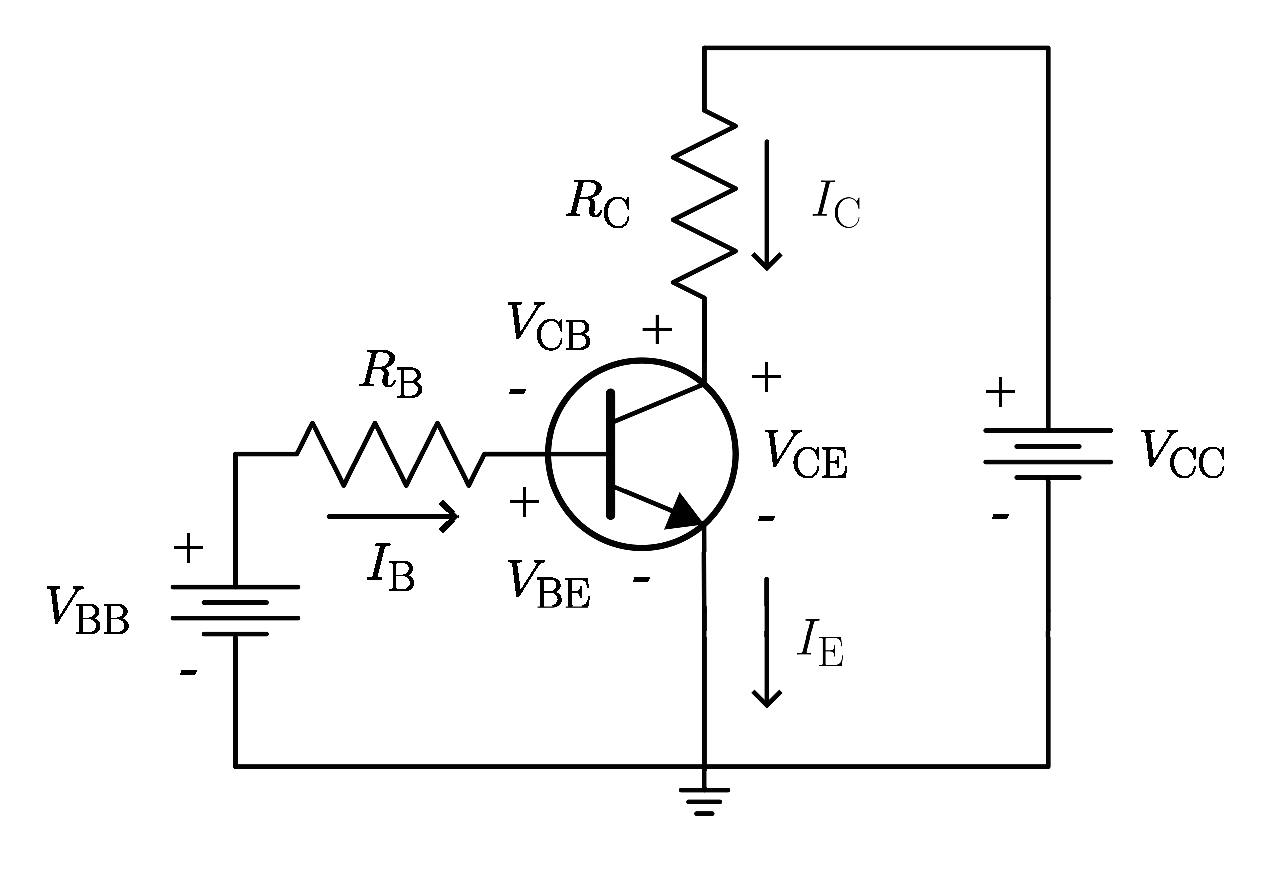
\includegraphics[scale=0.30]{diagramas/figura02.eps}
\caption{Circuito de polarización de cd del transistor \emph{npn}.}
\label{figura02}
\end{figure}

El transistor de unión bipolar presenta ganancia de corriente, lo cual se puede
utilizar para amplificar señales, la \textbf{ganancia} de corriente de cd de un
transistor es el cociente de la corriente de cd del colector ($I_{\text{C}}$)
entre la corriente de cd de la base ($I_{\text{B}}$) y se expresa como
\textbf{beta} de cd ($\beta_{\text{CD}}$).
\begin{equation*}
    \beta_{\text{CD}} = \frac{I_{\text{C}}}{I_{\text{B}}}
\end{equation*}

Existen inconvenientes en el diseño debido a las variaciones de $\beta$ por los
cambios de corriente en el transistor. Además, durante la fabricación del
transistor, se producen variaciones en el valor de beta dentro de un mismo lote
de producción. Por tanto, dos transistores fabricados al mismo tiempo tendrán
diferentes valores de $\beta$, aun en los mismos niveles de corriente
\cite{Savant}.

Cuando la unión base-emisor se polariza en directa, opera como un diodo
polarizado en directa y la caída de voltaje con polarización en directa nominal
es:
\begin{equation*}
    V_{\text{BE}} \cong 0.7 [\text{V}]
\end{equation*}

\subsubsection{Curva característica}
Como el transistor es un dispositivo no lineal, una forma de definir su
operación es usar una serie de curvas características que muestren como varia la
corriente en el colector, $I_{\text{C}}$, con el voltaje en el colector con
respecto al emisor, $V_{\text{CE}}$, con valores especificados de corriente de
base, $I_{\text{B}}$ como puede verse en la \textbf{figura~\ref{figura03}}.

Puede distinguirse la región activa, en esta región el transistor se encuentra
activado. En este modo de trabajo el voltaje que hay entre el emisor y el
colector ($V_{\text{CE}}$) se encuentra entre las regiones de saturación y
corte. La corriente de colector ($I_{\text{C}}$) depende principalmente de la
corriente de base ($I_{\text{B}}$), en esta región el transistor puede funcionar
como amplificador de señales.

\begin{figure}[!ht]
\centering
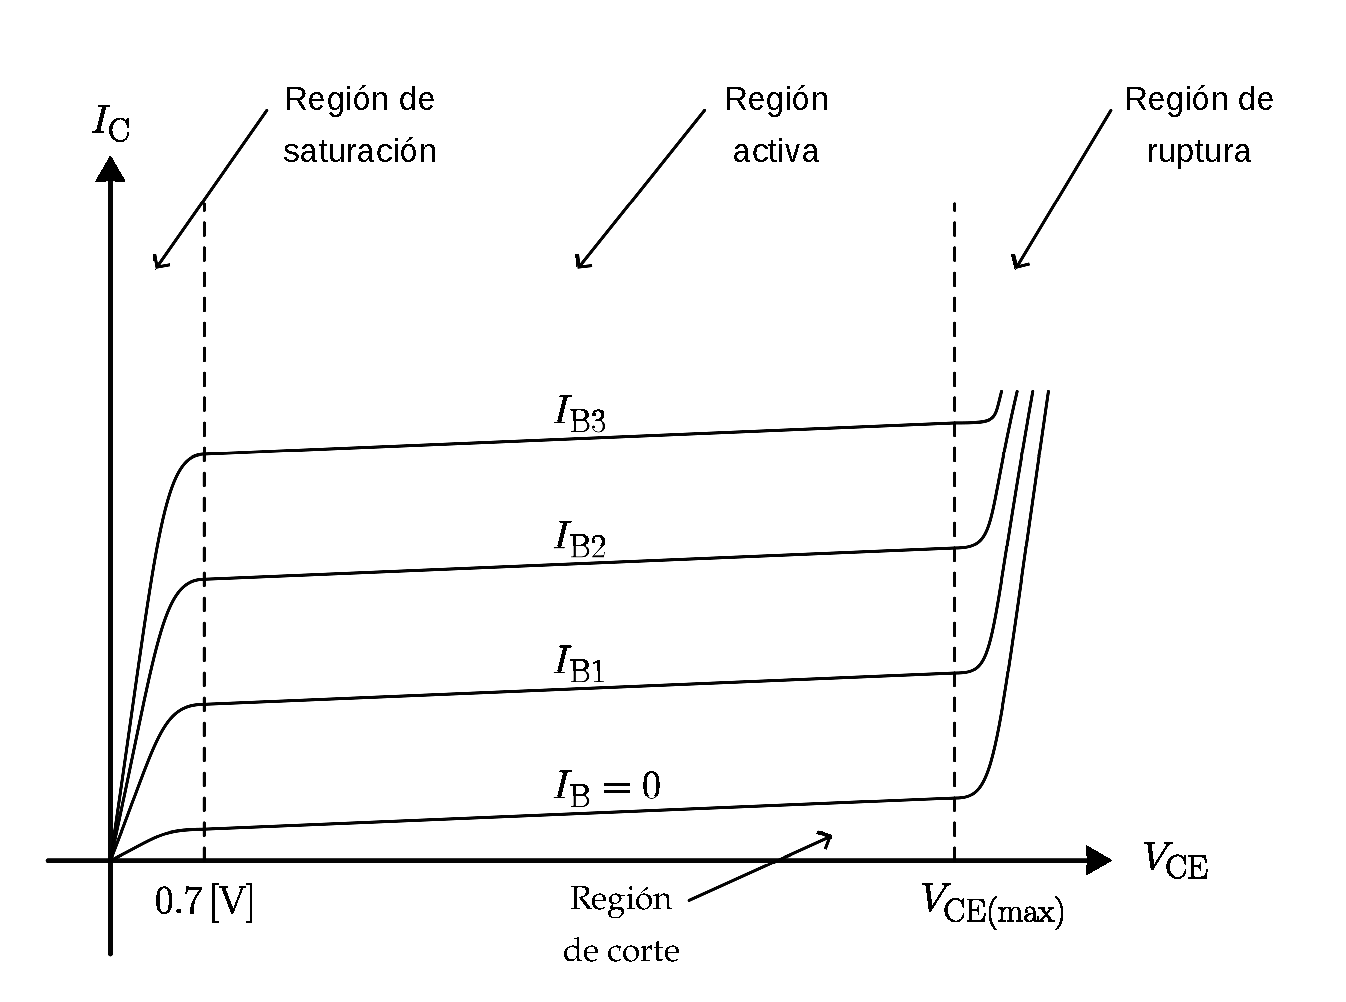
\includegraphics[scale=0.43]{diagramas/figura03.eps}
\caption{Familia de curvas $V_{\text{CE}}$ contra $I_{\text{C}}$ para varios
valores de $I_{\text{B}}$.}
\label{figura03}
\end{figure}

Un BJT, como cualquier otro dispositivo electrónico, tiene limitaciones en su
operación. Estas limitaciones se establecen en la forma de valores nominales
máximos y normalmente vienen especificadas en la hoja de datos del fabricante.
Típicamente se dan valores nominales máximos de voltaje en el colector con
respecto a la base, voltaje en el colector con respecto al emisor, voltaje en
el emisor con respecto a la base, corriente en el colector y disipación de
potencia.

El producto de $V_{\text{CE}}$ e $I_{\text{C}}$ no debe exceder la disipación de
potencia máxima. Tanto $V_{\text{CE}}$ como $I_{\text{C}}$ no pueden ser máximos
al mismo tiempo. Si $V_{\text{CE}}$ es máximo, $I_{\text{C}}$ se calcula como:
\begin{equation*}
    I_{\text{C}} = \frac{P_{\text{D(máx)}}}{V_{\text{CE}}}
\end{equation*}

\subsubsection{Transistor 2N2222A}
Para la construcción del amplificador se utilizará el transistor BJT tipo
\emph{npn} \textbf{2N2222A}; la hoja de datos de este transistor se detalla en
el \textbf{cuadro~\ref{cuadro01}} \cite{2N2222A}.

\begin{table}[!ht]
\begin{center}
    \begin{tabular}{|c|l|c|c|c|}
    \hline
    \multicolumn{5}{|c|}{\textbf{Valores nominales absolutos máximos}}
    \tabularnewline \hline
    \textbf{Símbolo} &
    \textbf{Parámetro} &
    \multicolumn{2}{|c|}{\textbf{Valor}} &
    \textbf{Unidades}
    \tabularnewline \hline \hline
    $V_{\text{CEO}}$ &
    Voltaje en colector-emisor &
    \multicolumn{2}{|c|}{$40$} & $V$
    \tabularnewline \hline
    $V_{\text{CBO}}$ &
    Voltaje en colector-base &
    \multicolumn{2}{|c|}{$75$} &
    $V$
    \tabularnewline \hline
    $V_{\text{EBO}}$ &
    Voltaje en emisor-base &
    \multicolumn{2}{|c|}{$6.0$} &
    $V$
    \tabularnewline \hline
    $I_{\text{C}}$ &
    Corriente en el colector &
    \multicolumn{2}{|c|}{$600$} &
    $mA$
    \tabularnewline \hline
    $P_{\text{D}}$ &
    Disipación total del dispositivo &
    \multicolumn{2}{|c|}{$625$} &
    $mW$
    \tabularnewline \hline \hline
    \multicolumn{5}{|c|}{\textbf{Características eléctricas (apagado)}}
    \tabularnewline \hline
    \textbf{Símbolo} &
    \textbf{Parámetro} &
    \textbf{Mín.} &
    \textbf{Máx.} &
    \textbf{Unidades}
    \tabularnewline \hline \hline
    $V_{\text{BR(CEO)}}$ &
    Voltaje de ruptura en colector-emisor &
    $40$ &
    $-$ &
    $V$
    \tabularnewline \hline
    $V_{\text{BR(CBO)}}$ &
    Voltaje de ruptura en colector-base &
    $75$ &
    $-$ &
    $V$
    \tabularnewline \hline
    $V_{\text{BR(EBO)}}$ &
    Voltaje de ruptura en emisor-base &
    $6.0$ &
    $-$ &
    $V$
    \tabularnewline \hline
    $I_{\text{CEX}}$ &
    Corriente de corte en el colector &
    $-$ &
    $10$ &
    $nA$
    \tabularnewline \hline
    $I_{\text{CBO}}$ &
    Corriente de corte en la base &
    $-$ &
    $10$ &
    $nA$
    \tabularnewline \hline
    $I_{\text{EBO}}$ &
    Corriente de corte en el emisor &
    $-$ &
    $10$ &
    $nA$
    \tabularnewline \hline \hline
    \multicolumn{5}{|c|}{\textbf{Características eléctricas (encendido)}}
    \tabularnewline \hline
    \textbf{Símbolo} &
    \textbf{Parámetro} &
    \textbf{Mín.} &
    \textbf{Máx.} &
    \textbf{Unidades}
    \tabularnewline \hline \hline
    $h_{\text{FE}}$ &
    Ganancia de corriente en CD & & & $-$
    \tabularnewline
    & $I_C = 0.1mA,\,V_{\text{CE}} = 10V$ &  $35$ &   $-$ & \tabularnewline
    & $I_C = 1.0mA,\,V_{\text{CE}} = 10V$ &  $50$ &   $-$ & \tabularnewline
    & $I_C =  10mA,\,V_{\text{CE}} = 10V$ &  $75$ &   $-$ & \tabularnewline
    & $I_C = 150mA,\,V_{\text{CE}} = 10V$ & $100$ & $300$ & \tabularnewline
    & $I_C = 500mA,\,V_{\text{CE}} = 10V$ &  $40$ &   $-$ &
    \tabularnewline \hline
    $V_{\text{CE(sat)}}$ &
    Voltaje de saturación en colector-emisor & & & $V$
    \tabularnewline
    & $I_C = 150mA,\,I_B = 15mA$ & $-$ & $0.3$ & \tabularnewline
    & $I_C = 500mA,\,I_B = 50mA$ & $-$ & $1.0$ &
    \tabularnewline \hline
    $V_{\text{BE(sat)}}$ &
    Voltaje de saturación en base-emisor & & & $V$
    \tabularnewline
    & $I_C = 150mA,\,I_B = 15mA$ & $-$ & $1.2$ & \tabularnewline
    & $I_C = 500mA,\,I_B = 50mA$ & $-$ & $2.0$ &
    \tabularnewline \hline
    \end{tabular}
\end{center}
\caption{Hoja de datos parcial 2N2222A.}
\label{cuadro01}
\end{table}

\subsubsection{Medición de transistores}
Como se mencionó anteriormente la ganancia de los transistores BJT varían en un
intervalo amplio, por lo cual es recomendable medir individualmente cada uno,
para los cálculos del amplificador.

Se cuenta con un lote de 40 transistores 2N2222A como puede verse en la
\textbf{figura~\ref{figura04}}. Las ganancias ($h_{\text{FE}}$) medidas con un
multímetro en los transistores se detallan en el \textbf{cuadro~\ref{cuadro02}}.

\begin{figure}[!ht]
\centering
\includegraphics[scale=0.12]{diagramas/figura04.eps}
\caption{Lote de transistores 2N2222A.}
\label{figura04}
\end{figure}

\begin{table}[!ht]
\begin{center}
    \begin{tabular}{|c|c|c|c|c|c|c|c|c|c|}
    \hline
    \multicolumn{10}{|c|}{\textbf{$h_{\text{FE}}$}}
    \tabularnewline \hline \hline
    253 & 256 & 297 & 302 & 304 & 264 & 282 & 250 & 279 & 257
    \tabularnewline \hline
    253 & 255 & 289 & 261 & 272 & 282 & 294 & 260 & 264 & 297
    \tabularnewline \hline
    303 & 297 & 280 & 278 & 257 & 255 & 266 & 300 & 295 & 291
    \tabularnewline \hline
    272 & 279 & 262 & 266 & 256 & 285 & 257 & 267 & 289 & 268
    \tabularnewline \hline
    \end{tabular}
\end{center}
\caption{Valor de ganancia medido de cada transistor del lote.}
\label{cuadro02}
\end{table}

La distribución de frecuencias se muestra en la \textbf{figura~\ref{figura05}};
de los cuales se escogieron los tres transistores con mayor valor de ganancia.

\begin{figure}[!ht]
\centering
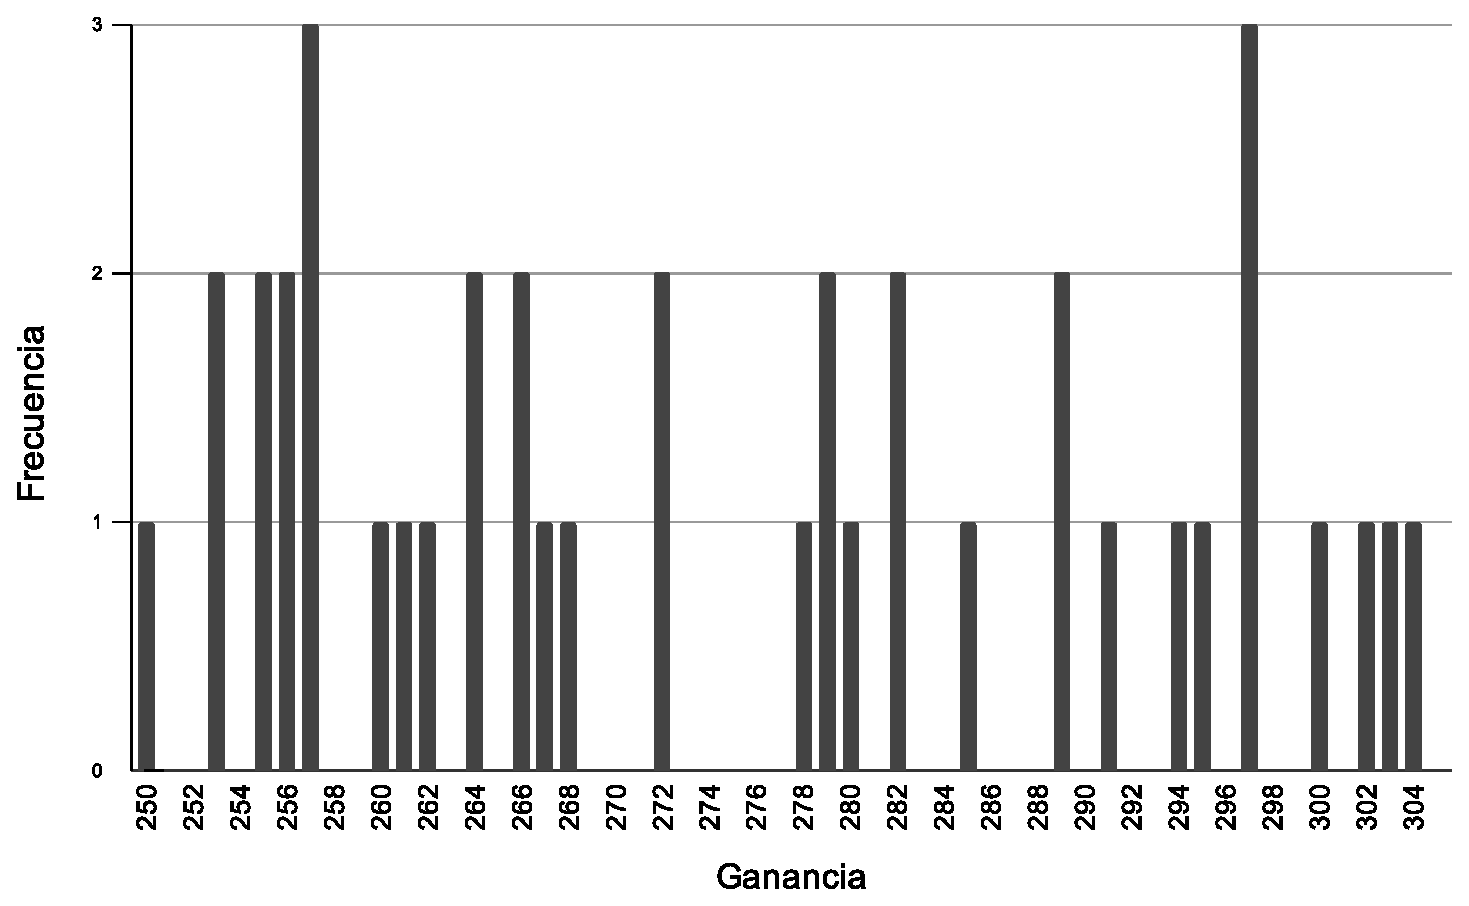
\includegraphics[scale=0.5]{diagramas/figura05.eps}
\caption{Distribución de frecuencia de ganancias de los transistores.}
\label{figura05}
\end{figure}

Por tanto, los transistores a utilizar tienen los parametros descritos en el
\textbf{cuadro~\ref{cuadro03}}.

\begin{table}[!ht]
\begin{center}
    \begin{tabular}{|c||c|c|}
    \hline
    No. & $h_{\text{FE}}$ & $V_{\text{BE}}\,[V]$
    \tabularnewline \hline \hline
    1 & 302 & 0.675
    \tabularnewline \hline
    2 & 303 & 0.676
    \tabularnewline \hline
    3 & 304 & 0.676
    \tabularnewline \hline
    \end{tabular}
\end{center}
\caption{Valores $h_{\text{FE}}$ y $V_{\text{BE}}$ medidos en los transistores.}
\label{cuadro03}
\end{table}


%\subsection{FET}
El transistor JFET (transistor de efecto de campo de unión) es un tipo de FET
que opera con una unión \emph{pn} polarizada en inversa para controlar corriente
en un canal. Según su estructura, los JFET caen dentro de cualquiera de dos
categorías, de canal \emph{n} o de canal \emph{p}. Cada extremo del canal tiene
una terminal; el \textbf{drenaje} se encuentra en el extremo superior y la
\textbf{fuente} en el inferior. Se forma un canal donde se conecta la terminal
de la \textbf{compuerta} como se muestra en la \textbf{figura~\ref{figura06}}
junto a sus símbolos esquemáticos \cite{Floyd}.

\begin{figure}[!ht]
\centering
\includegraphics[scale=0.30]{diagramas/figura06.eps}
\caption{Tipos de transistores JFET y sus símbolos estándar.}
\label{figura06}
\end{figure}

Ambos tipos de FET se controlan por una tensión entre la compuerta y la fuente.
La fuente y el drenaje de un FET se pueden intercambiar sin afectar la operación
del transistor.

Cuando se conecta un transistor JFET a un circuito, como se muestra en la
\textbf{figura~\ref{figura07}}, se aplica una fuente de tensión $V_{\text{DD}}$
al drenaje (análoga a la fuente de tensión $V_{\text{CC}}$ para el BJT) y se
envía a tierra. Una fuente de tensión de compuerta $V_{\text{GG}}$ se aplica a
la compuerta (análoga a $V_{\text{BB}}$ para el BJT).

$V_{\text{DD}}$ proporciona una tensión drenaje a fuente $V_{\text{DS}}$ que
provoca una corriente de drenaje $I_{\text{D}}$ del drenaje a la fuente. La
corriente de drenaje $I_{\text{D}}$ que es idéntica a la corriente de fuente,
existe en el canal rodeado por la compuerta de tipo \emph{p}. La tensión
compuerta a fuente $V_{\text{GS}}$ que es igual a $-V_{\text{GG}}$ crea una
región desértica en el canal que reduce el ancho de este y por tanto aumenta la
resistencia entre drenaje y fuente. Como la unión compuerta-fuente esta
polarizada en inverso, el resultado es una corriente de compuerta nula
\cite{Savant}.

\begin{figure}[!ht]
\centering
\includegraphics[scale=0.30]{diagramas/figura07.eps}
\caption{Circuito de polarización de cd del transistor canal \emph{n}.}
\label{figura07}
\end{figure}

Cuando se incrementa $V_{\text{DS}}$ también aumenta la corriente de drenaje
$I_{\text{D}}$, conforme aumenta $V_{\text{DS}}$ se alcanza un punto donde la
corriente de drenaje alcanza su punto de saturación. Si se aumenta
$V_{\text{DS}}$ mas allá de este punto $I_{\text{D}}$ permanece constante. El
valor de la corriente de saturación de drenaje con $V_{\text{GS}} = 0$ es un
parámetro importante y se denomina \textbf{corriente de drenaje de saturación}
($I_{\text{DSS}}$).

El FET es un dispositivo controlado por tensión y se controla mediante
$V_{\text{GS}}$. Conforme se incrementa $V_{\text{GS}}$ (más negativo para un
canal \emph{n} y más positivo para un canal \emph{p}) se cierra para un valor
menor que $I_{\text{D}}$. Por tanto, para el JFET de canal \emph{n} la
$I_{\text{D}}$ máxima se reduce desde $I_{\text{DSS}}$ conforme $V_{\text{GS}}$
se hace mas negativo. Si $V_{\text{GS}}$ disminuye aun mas (mas negativo), se
alcanza un valor de $V_{\text{GS}}$ después del cual $I_{\text{D}}$ sera cero
sin importar el valor de $V_{\text{DS}}$. Este valor de $V_{\text{GS}}$ se
denomina $V_{\text{GS(corte)}}$ o \textbf{tensión de estrangulamiento}
($V_{\text{p}}$). El valor de $V_{\text{p}}$ es negativo para un JFET de canal
\emph{n} y positivo para un JFET de canal \emph{p} \cite{Savant}.

\subsubsection{Curva característica}
En la \textbf{figura~\ref{figura08}} se muestran las curvas características de
transferencia y la curva característica $I_{\text{D}}-V_{\text{GS}}$ para un
JFET de canal \emph{n}. Se graficaron con el eje $I_{\text{D}}$ común.

\begin{figure}[!ht]
\centering
\includegraphics[scale=0.43]{diagramas/figura08.eps}
\caption{Familia de curvas $V_{\text{CE}}$ contra $I_{\text{C}}$ para varios
valores de $I_{\text{B}}$.}
\label{figura08}
\end{figure}

Un método útil de determinar la curva característica de transferencia es con
ayuda de la siguiente relación (ecuación de \emph{Shockley}):

\begin{equation*}
    \frac{I_{\text{D}}}{I_{\text{DSS}}} \approx
    \left(1 - \frac{V_{\text{GS}}}{V_{\text{p}}}\right)^2
\end{equation*}

Por tanto, solo se necesita conocer $I_{\text{DSS}}$ y $V_{\text{p}}$, y toda la
característica queda determinada.

\subsubsection{Transistor 2N3819}
Para la construcción del amplificador se utilizará el transistor JFET canal
\emph{n} \textbf{2N3819}; la hoja de datos de este transistor se detalla en
el \textbf{cuadro~\ref{cuadro04}} \cite{2N3819}.

\begin{table}[!ht]
\begin{center}
    \begin{tabular}{|c|l|c|c|c|}
    \hline
    \multicolumn{5}{|c|}{\textbf{Valores nominales absolutos máximos}}
    \tabularnewline \hline
    \textbf{Símbolo} &
    \textbf{Parámetro} &
    \multicolumn{2}{|c|}{\textbf{Valor}} &
    \textbf{Unidades}
    \tabularnewline \hline \hline
    $V_{\text{DG}}$ &
    Voltaje drenaje-compuerta &
    \multicolumn{2}{|c|}{$25$} & $V$
    \tabularnewline \hline
    $V_{\text{GS}}$ &
    Voltaje compuerta-fuente &
    \multicolumn{2}{|c|}{$-25$} &
    $V$
    \tabularnewline \hline
    $I_{\text{D}}$ &
    Corriente de drenaje &
    \multicolumn{2}{|c|}{$50$} &
    $mA$
    \tabularnewline \hline
    $I_{\text{GF}}$ &
    Corriente en compuerta en polarización directa &
    \multicolumn{2}{|c|}{$10$} &
    $mA$
    \tabularnewline \hline
    $P_{\text{D}}$ &
    Disipación total del dispositivo &
    \multicolumn{2}{|c|}{$350$} &
    $mW$
    \tabularnewline \hline \hline
    \multicolumn{5}{|c|}{\textbf{Características eléctricas (apagado)}}
    \tabularnewline \hline
    \textbf{Símbolo} &
    \textbf{Parámetro} &
    \textbf{Mín.} &
    \textbf{Máx.} &
    \textbf{Unidades}
    \tabularnewline \hline \hline
    $V_{\text{BR(GSS)}}$ &
    Voltaje de ruptura entre compuerta y fuente &
    $25$ &
    $-$ &
    $V$
    \tabularnewline \hline
    $I_{\text{GSS}}$ &
    Corriente inversa en la compuerta &
    $-$ &
    $2.0$ &
    $nA$
    \tabularnewline \hline
    $V_{\text{GS(off)}}$ &
    Voltaje de corte entre compuerta y fuente &
    $-$ &
    $8$ &
    $V$
    \tabularnewline \hline
    $V_{\text{GS}}$ &
    Voltaje entre la compuerta y fuente &
    $-0.5$ &
    $-7.5$ &
    $V$
    \tabularnewline \hline \hline
    \multicolumn{5}{|c|}{\textbf{Características eléctricas (encendido)}}
    \tabularnewline \hline
    \textbf{Símbolo} &
    \textbf{Parámetro} &
    \textbf{Mín.} &
    \textbf{Máx.} &
    \textbf{Unidades}
    \tabularnewline \hline \hline
    $I_{\text{DSS}}$ &
    Corriente en drenaje con voltaje cero en compuerta &
    $2$ &
    $20$ &
    $mA$
    \tabularnewline \hline
    \end{tabular}
\end{center}
\caption{Hoja de datos parcial 2N3819.}
\label{cuadro04}
\end{table}

\subsubsection{Medición de transistores}
Como en el caso de los transistores BJT, los transistores JFET pueden variar sus
parámetros individualmente en un intervalo determinado por la hoja de datos.

\begin{figure}[!ht]
\centering
\includegraphics[scale=0.04]{diagramas/figura09.eps}
\caption{Transistores 2N3918.}
\label{figura09}
\end{figure}

Debido al alto costo de los transistores JFET solo se cuentan con tres de ellos
como puede verse en la \textbf{figura~\ref{figura09}}, de los cuales se medirán
su corriente de drenaje de saturación ($I_{\text{DSS}}$) y su tensión de
estrangulamiento ($V_{\text{p}}$), con la ayuda del circuito presentado en la
\textbf{figura~\ref{figura10}} \cite{measuring}.

\begin{figure}[!ht]
\centering
\includegraphics[scale=0.30]{diagramas/figura10.eps}
\caption{Circuito para el calculo de $V_{\text{p}}$ y $I_{\text{DSS}}$.}
\label{figura10}
\end{figure}

Los valores obtenidos en la medición son detallados en el
\textbf{cuadro~\ref{cuadro05}} con los cuales pueden hallarse las curvas
características que pueden verse en la \textbf{figura~\ref{curva01}}.

\begin{table}[!ht]
\begin{center}
    \begin{tabular}{|c||c|c|}
    \hline
    No. & $V_{\text{p}}\,[V]$ & $I_{\text{DSS}}\,[mA]$
    \tabularnewline \hline \hline
    1 & -1.037 & 15.8
    \tabularnewline \hline
    2 & -1.098 & 17.7
    \tabularnewline \hline
    3 & -1.135 & 18.5
    \tabularnewline \hline
    \end{tabular}
\end{center}
\caption{Valores $V_{\text{p}}$ y $I_{\text{DSS}}$ medidos en los transistores.}
\label{cuadro05}
\end{table}

\begin{figure}[!ht]
    \centering
    % GNUPLOT: LaTeX picture with Postscript
\begingroup
  \makeatletter
  \providecommand\color[2][]{%
    \GenericError{(gnuplot) \space\space\space\@spaces}{%
      Package color not loaded in conjunction with
      terminal option `colourtext'%
    }{See the gnuplot documentation for explanation.%
    }{Either use 'blacktext' in gnuplot or load the package
      color.sty in LaTeX.}%
    \renewcommand\color[2][]{}%
  }%
  \providecommand\includegraphics[2][]{%
    \GenericError{(gnuplot) \space\space\space\@spaces}{%
      Package graphicx or graphics not loaded%
    }{See the gnuplot documentation for explanation.%
    }{The gnuplot epslatex terminal needs graphicx.sty or graphics.sty.}%
    \renewcommand\includegraphics[2][]{}%
  }%
  \providecommand\rotatebox[2]{#2}%
  \@ifundefined{ifGPcolor}{%
    \newif\ifGPcolor
    \GPcolorfalse
  }{}%
  \@ifundefined{ifGPblacktext}{%
    \newif\ifGPblacktext
    \GPblacktexttrue
  }{}%
  % define a \g@addto@macro without @ in the name:
  \let\gplgaddtomacro\g@addto@macro
  % define empty templates for all commands taking text:
  \gdef\gplbacktext{}%
  \gdef\gplfronttext{}%
  \makeatother
  \ifGPblacktext
    % no textcolor at all
    \def\colorrgb#1{}%
    \def\colorgray#1{}%
  \else
    % gray or color?
    \ifGPcolor
      \def\colorrgb#1{\color[rgb]{#1}}%
      \def\colorgray#1{\color[gray]{#1}}%
      \expandafter\def\csname LTw\endcsname{\color{white}}%
      \expandafter\def\csname LTb\endcsname{\color{black}}%
      \expandafter\def\csname LTa\endcsname{\color{black}}%
      \expandafter\def\csname LT0\endcsname{\color[rgb]{1,0,0}}%
      \expandafter\def\csname LT1\endcsname{\color[rgb]{0,1,0}}%
      \expandafter\def\csname LT2\endcsname{\color[rgb]{0,0,1}}%
      \expandafter\def\csname LT3\endcsname{\color[rgb]{1,0,1}}%
      \expandafter\def\csname LT4\endcsname{\color[rgb]{0,1,1}}%
      \expandafter\def\csname LT5\endcsname{\color[rgb]{1,1,0}}%
      \expandafter\def\csname LT6\endcsname{\color[rgb]{0,0,0}}%
      \expandafter\def\csname LT7\endcsname{\color[rgb]{1,0.3,0}}%
      \expandafter\def\csname LT8\endcsname{\color[rgb]{0.5,0.5,0.5}}%
    \else
      % gray
      \def\colorrgb#1{\color{black}}%
      \def\colorgray#1{\color[gray]{#1}}%
      \expandafter\def\csname LTw\endcsname{\color{white}}%
      \expandafter\def\csname LTb\endcsname{\color{black}}%
      \expandafter\def\csname LTa\endcsname{\color{black}}%
      \expandafter\def\csname LT0\endcsname{\color{black}}%
      \expandafter\def\csname LT1\endcsname{\color{black}}%
      \expandafter\def\csname LT2\endcsname{\color{black}}%
      \expandafter\def\csname LT3\endcsname{\color{black}}%
      \expandafter\def\csname LT4\endcsname{\color{black}}%
      \expandafter\def\csname LT5\endcsname{\color{black}}%
      \expandafter\def\csname LT6\endcsname{\color{black}}%
      \expandafter\def\csname LT7\endcsname{\color{black}}%
      \expandafter\def\csname LT8\endcsname{\color{black}}%
    \fi
  \fi
    \setlength{\unitlength}{0.0500bp}%
    \ifx\gptboxheight\undefined%
      \newlength{\gptboxheight}%
      \newlength{\gptboxwidth}%
      \newsavebox{\gptboxtext}%
    \fi%
    \setlength{\fboxrule}{0.5pt}%
    \setlength{\fboxsep}{1pt}%
    \definecolor{tbcol}{rgb}{1,1,1}%
\begin{picture}(6336.00,4030.00)%
    \gplgaddtomacro\gplbacktext{%
      \csname LTb\endcsname%%
      \put(5855,440){\makebox(0,0)[r]{\strut{}}}%
      \csname LTb\endcsname%%
      \put(5855,609){\makebox(0,0)[r]{\strut{}}}%
      \csname LTb\endcsname%%
      \put(5855,779){\makebox(0,0)[r]{\strut{}}}%
      \csname LTb\endcsname%%
      \put(5855,948){\makebox(0,0)[r]{\strut{}}}%
      \csname LTb\endcsname%%
      \put(5855,1118){\makebox(0,0)[r]{\strut{}}}%
      \csname LTb\endcsname%%
      \put(5855,1287){\makebox(0,0)[r]{\strut{}}}%
      \csname LTb\endcsname%%
      \put(5855,1457){\makebox(0,0)[r]{\strut{}}}%
      \csname LTb\endcsname%%
      \put(5855,1626){\makebox(0,0)[r]{\strut{}}}%
      \csname LTb\endcsname%%
      \put(5855,1796){\makebox(0,0)[r]{\strut{}}}%
      \csname LTb\endcsname%%
      \put(5855,1965){\makebox(0,0)[r]{\strut{}}}%
      \csname LTb\endcsname%%
      \put(5855,2135){\makebox(0,0)[r]{\strut{}}}%
      \csname LTb\endcsname%%
      \put(5855,2304){\makebox(0,0)[r]{\strut{}}}%
      \csname LTb\endcsname%%
      \put(5855,2473){\makebox(0,0)[r]{\strut{}}}%
      \csname LTb\endcsname%%
      \put(5855,2643){\makebox(0,0)[r]{\strut{}}}%
      \csname LTb\endcsname%%
      \put(5855,2812){\makebox(0,0)[r]{\strut{}}}%
      \csname LTb\endcsname%%
      \put(5855,2982){\makebox(0,0)[r]{\strut{}}}%
      \csname LTb\endcsname%%
      \put(5855,3151){\makebox(0,0)[r]{\strut{}}}%
      \csname LTb\endcsname%%
      \put(5855,3321){\makebox(0,0)[r]{\strut{}}}%
      \csname LTb\endcsname%%
      \put(5855,3490){\makebox(0,0)[r]{\strut{}}}%
      \csname LTb\endcsname%%
      \put(5855,3660){\makebox(0,0)[r]{\strut{}}}%
      \csname LTb\endcsname%%
      \put(5855,3829){\makebox(0,0)[r]{\strut{}}}%
      \csname LTb\endcsname%%
      \put(500,240){\makebox(0,0){\strut{}}}%
      \csname LTb\endcsname%%
      \put(956,240){\makebox(0,0){\strut{}}}%
      \csname LTb\endcsname%%
      \put(1412,240){\makebox(0,0){\strut{}}}%
      \csname LTb\endcsname%%
      \put(1869,240){\makebox(0,0){\strut{}}}%
      \csname LTb\endcsname%%
      \put(2325,240){\makebox(0,0){\strut{}}}%
      \csname LTb\endcsname%%
      \put(2781,240){\makebox(0,0){\strut{}}}%
      \csname LTb\endcsname%%
      \put(3237,240){\makebox(0,0){\strut{}}}%
      \csname LTb\endcsname%%
      \put(3694,240){\makebox(0,0){\strut{}}}%
      \csname LTb\endcsname%%
      \put(4150,240){\makebox(0,0){\strut{}}}%
      \csname LTb\endcsname%%
      \put(4606,240){\makebox(0,0){\strut{}}}%
      \csname LTb\endcsname%%
      \put(5062,240){\makebox(0,0){\strut{}}}%
      \csname LTb\endcsname%%
      \put(5519,240){\makebox(0,0){\strut{}}}%
      \csname LTb\endcsname%%
      \put(5975,240){\makebox(0,0){\strut{}}}%
      \csname LTb\endcsname%%
      \put(500,271){\makebox(0,0)[l]{\strut{}-1.135}}%
      \put(1184,271){\makebox(0,0)[l]{\strut{}-1.098}}%
      \put(1869,271){\makebox(0,0)[l]{\strut{}-1.037}}%
      \put(6112,3575){\makebox(0,0)[l]{\strut{}18.5}}%
      \put(6112,3405){\makebox(0,0)[l]{\strut{}17.7}}%
      \put(6112,3151){\makebox(0,0)[l]{\strut{}15.8}}%
    }%
    \gplgaddtomacro\gplfronttext{%
      \csname LTb\endcsname%%
      \put(190,2134){\rotatebox{-270.00}{\makebox(0,0){\strut{}$I_{\text{D}}[mA]$}}}%
      \put(3237,140){\makebox(0,0){\strut{}$V_{\text{GS}}[V]$}}%
    }%
    \gplgaddtomacro\gplbacktext{%
      \csname LTb\endcsname%%
      \put(5855,440){\makebox(0,0)[r]{\strut{}}}%
      \csname LTb\endcsname%%
      \put(5855,609){\makebox(0,0)[r]{\strut{}}}%
      \csname LTb\endcsname%%
      \put(5855,779){\makebox(0,0)[r]{\strut{}}}%
      \csname LTb\endcsname%%
      \put(5855,948){\makebox(0,0)[r]{\strut{}}}%
      \csname LTb\endcsname%%
      \put(5855,1118){\makebox(0,0)[r]{\strut{}}}%
      \csname LTb\endcsname%%
      \put(5855,1287){\makebox(0,0)[r]{\strut{}}}%
      \csname LTb\endcsname%%
      \put(5855,1457){\makebox(0,0)[r]{\strut{}}}%
      \csname LTb\endcsname%%
      \put(5855,1626){\makebox(0,0)[r]{\strut{}}}%
      \csname LTb\endcsname%%
      \put(5855,1796){\makebox(0,0)[r]{\strut{}}}%
      \csname LTb\endcsname%%
      \put(5855,1965){\makebox(0,0)[r]{\strut{}}}%
      \csname LTb\endcsname%%
      \put(5855,2135){\makebox(0,0)[r]{\strut{}}}%
      \csname LTb\endcsname%%
      \put(5855,2304){\makebox(0,0)[r]{\strut{}}}%
      \csname LTb\endcsname%%
      \put(5855,2473){\makebox(0,0)[r]{\strut{}}}%
      \csname LTb\endcsname%%
      \put(5855,2643){\makebox(0,0)[r]{\strut{}}}%
      \csname LTb\endcsname%%
      \put(5855,2812){\makebox(0,0)[r]{\strut{}}}%
      \csname LTb\endcsname%%
      \put(5855,2982){\makebox(0,0)[r]{\strut{}}}%
      \csname LTb\endcsname%%
      \put(5855,3151){\makebox(0,0)[r]{\strut{}}}%
      \csname LTb\endcsname%%
      \put(5855,3321){\makebox(0,0)[r]{\strut{}}}%
      \csname LTb\endcsname%%
      \put(5855,3490){\makebox(0,0)[r]{\strut{}}}%
      \csname LTb\endcsname%%
      \put(5855,3660){\makebox(0,0)[r]{\strut{}}}%
      \csname LTb\endcsname%%
      \put(5855,3829){\makebox(0,0)[r]{\strut{}}}%
      \csname LTb\endcsname%%
      \put(500,240){\makebox(0,0){\strut{}}}%
      \csname LTb\endcsname%%
      \put(956,240){\makebox(0,0){\strut{}}}%
      \csname LTb\endcsname%%
      \put(1412,240){\makebox(0,0){\strut{}}}%
      \csname LTb\endcsname%%
      \put(1869,240){\makebox(0,0){\strut{}}}%
      \csname LTb\endcsname%%
      \put(2325,240){\makebox(0,0){\strut{}}}%
      \csname LTb\endcsname%%
      \put(2781,240){\makebox(0,0){\strut{}}}%
      \csname LTb\endcsname%%
      \put(3237,240){\makebox(0,0){\strut{}}}%
      \csname LTb\endcsname%%
      \put(3694,240){\makebox(0,0){\strut{}}}%
      \csname LTb\endcsname%%
      \put(4150,240){\makebox(0,0){\strut{}}}%
      \csname LTb\endcsname%%
      \put(4606,240){\makebox(0,0){\strut{}}}%
      \csname LTb\endcsname%%
      \put(5062,240){\makebox(0,0){\strut{}}}%
      \csname LTb\endcsname%%
      \put(5519,240){\makebox(0,0){\strut{}}}%
      \csname LTb\endcsname%%
      \put(5975,240){\makebox(0,0){\strut{}}}%
      \csname LTb\endcsname%%
      \put(500,271){\makebox(0,0)[l]{\strut{}-1.135}}%
      \put(1184,271){\makebox(0,0)[l]{\strut{}-1.098}}%
      \put(1869,271){\makebox(0,0)[l]{\strut{}-1.037}}%
      \put(6112,3575){\makebox(0,0)[l]{\strut{}18.5}}%
      \put(6112,3405){\makebox(0,0)[l]{\strut{}17.7}}%
      \put(6112,3151){\makebox(0,0)[l]{\strut{}15.8}}%
    }%
    \gplgaddtomacro\gplfronttext{%
      \csname LTb\endcsname%%
      \put(190,2134){\rotatebox{-270.00}{\makebox(0,0){\strut{}$I_{\text{D}}[mA]$}}}%
      \put(3237,140){\makebox(0,0){\strut{}$V_{\text{GS}}[V]$}}%
    }%
    \gplgaddtomacro\gplbacktext{%
      \csname LTb\endcsname%%
      \put(5855,440){\makebox(0,0)[r]{\strut{}}}%
      \csname LTb\endcsname%%
      \put(5855,609){\makebox(0,0)[r]{\strut{}}}%
      \csname LTb\endcsname%%
      \put(5855,779){\makebox(0,0)[r]{\strut{}}}%
      \csname LTb\endcsname%%
      \put(5855,948){\makebox(0,0)[r]{\strut{}}}%
      \csname LTb\endcsname%%
      \put(5855,1118){\makebox(0,0)[r]{\strut{}}}%
      \csname LTb\endcsname%%
      \put(5855,1287){\makebox(0,0)[r]{\strut{}}}%
      \csname LTb\endcsname%%
      \put(5855,1457){\makebox(0,0)[r]{\strut{}}}%
      \csname LTb\endcsname%%
      \put(5855,1626){\makebox(0,0)[r]{\strut{}}}%
      \csname LTb\endcsname%%
      \put(5855,1796){\makebox(0,0)[r]{\strut{}}}%
      \csname LTb\endcsname%%
      \put(5855,1965){\makebox(0,0)[r]{\strut{}}}%
      \csname LTb\endcsname%%
      \put(5855,2135){\makebox(0,0)[r]{\strut{}}}%
      \csname LTb\endcsname%%
      \put(5855,2304){\makebox(0,0)[r]{\strut{}}}%
      \csname LTb\endcsname%%
      \put(5855,2473){\makebox(0,0)[r]{\strut{}}}%
      \csname LTb\endcsname%%
      \put(5855,2643){\makebox(0,0)[r]{\strut{}}}%
      \csname LTb\endcsname%%
      \put(5855,2812){\makebox(0,0)[r]{\strut{}}}%
      \csname LTb\endcsname%%
      \put(5855,2982){\makebox(0,0)[r]{\strut{}}}%
      \csname LTb\endcsname%%
      \put(5855,3151){\makebox(0,0)[r]{\strut{}}}%
      \csname LTb\endcsname%%
      \put(5855,3321){\makebox(0,0)[r]{\strut{}}}%
      \csname LTb\endcsname%%
      \put(5855,3490){\makebox(0,0)[r]{\strut{}}}%
      \csname LTb\endcsname%%
      \put(5855,3660){\makebox(0,0)[r]{\strut{}}}%
      \csname LTb\endcsname%%
      \put(5855,3829){\makebox(0,0)[r]{\strut{}}}%
      \csname LTb\endcsname%%
      \put(500,240){\makebox(0,0){\strut{}}}%
      \csname LTb\endcsname%%
      \put(956,240){\makebox(0,0){\strut{}}}%
      \csname LTb\endcsname%%
      \put(1412,240){\makebox(0,0){\strut{}}}%
      \csname LTb\endcsname%%
      \put(1869,240){\makebox(0,0){\strut{}}}%
      \csname LTb\endcsname%%
      \put(2325,240){\makebox(0,0){\strut{}}}%
      \csname LTb\endcsname%%
      \put(2781,240){\makebox(0,0){\strut{}}}%
      \csname LTb\endcsname%%
      \put(3237,240){\makebox(0,0){\strut{}}}%
      \csname LTb\endcsname%%
      \put(3694,240){\makebox(0,0){\strut{}}}%
      \csname LTb\endcsname%%
      \put(4150,240){\makebox(0,0){\strut{}}}%
      \csname LTb\endcsname%%
      \put(4606,240){\makebox(0,0){\strut{}}}%
      \csname LTb\endcsname%%
      \put(5062,240){\makebox(0,0){\strut{}}}%
      \csname LTb\endcsname%%
      \put(5519,240){\makebox(0,0){\strut{}}}%
      \csname LTb\endcsname%%
      \put(5975,240){\makebox(0,0){\strut{}}}%
      \csname LTb\endcsname%%
      \put(500,271){\makebox(0,0)[l]{\strut{}-1.135}}%
      \put(1184,271){\makebox(0,0)[l]{\strut{}-1.098}}%
      \put(1869,271){\makebox(0,0)[l]{\strut{}-1.037}}%
      \put(6112,3575){\makebox(0,0)[l]{\strut{}18.5}}%
      \put(6112,3405){\makebox(0,0)[l]{\strut{}17.7}}%
      \put(6112,3151){\makebox(0,0)[l]{\strut{}15.8}}%
    }%
    \gplgaddtomacro\gplfronttext{%
      \csname LTb\endcsname%%
      \put(190,2134){\rotatebox{-270.00}{\makebox(0,0){\strut{}$I_{\text{D}}[mA]$}}}%
      \put(3237,140){\makebox(0,0){\strut{}$V_{\text{GS}}[V]$}}%
    }%
    \gplbacktext
    \put(0,0){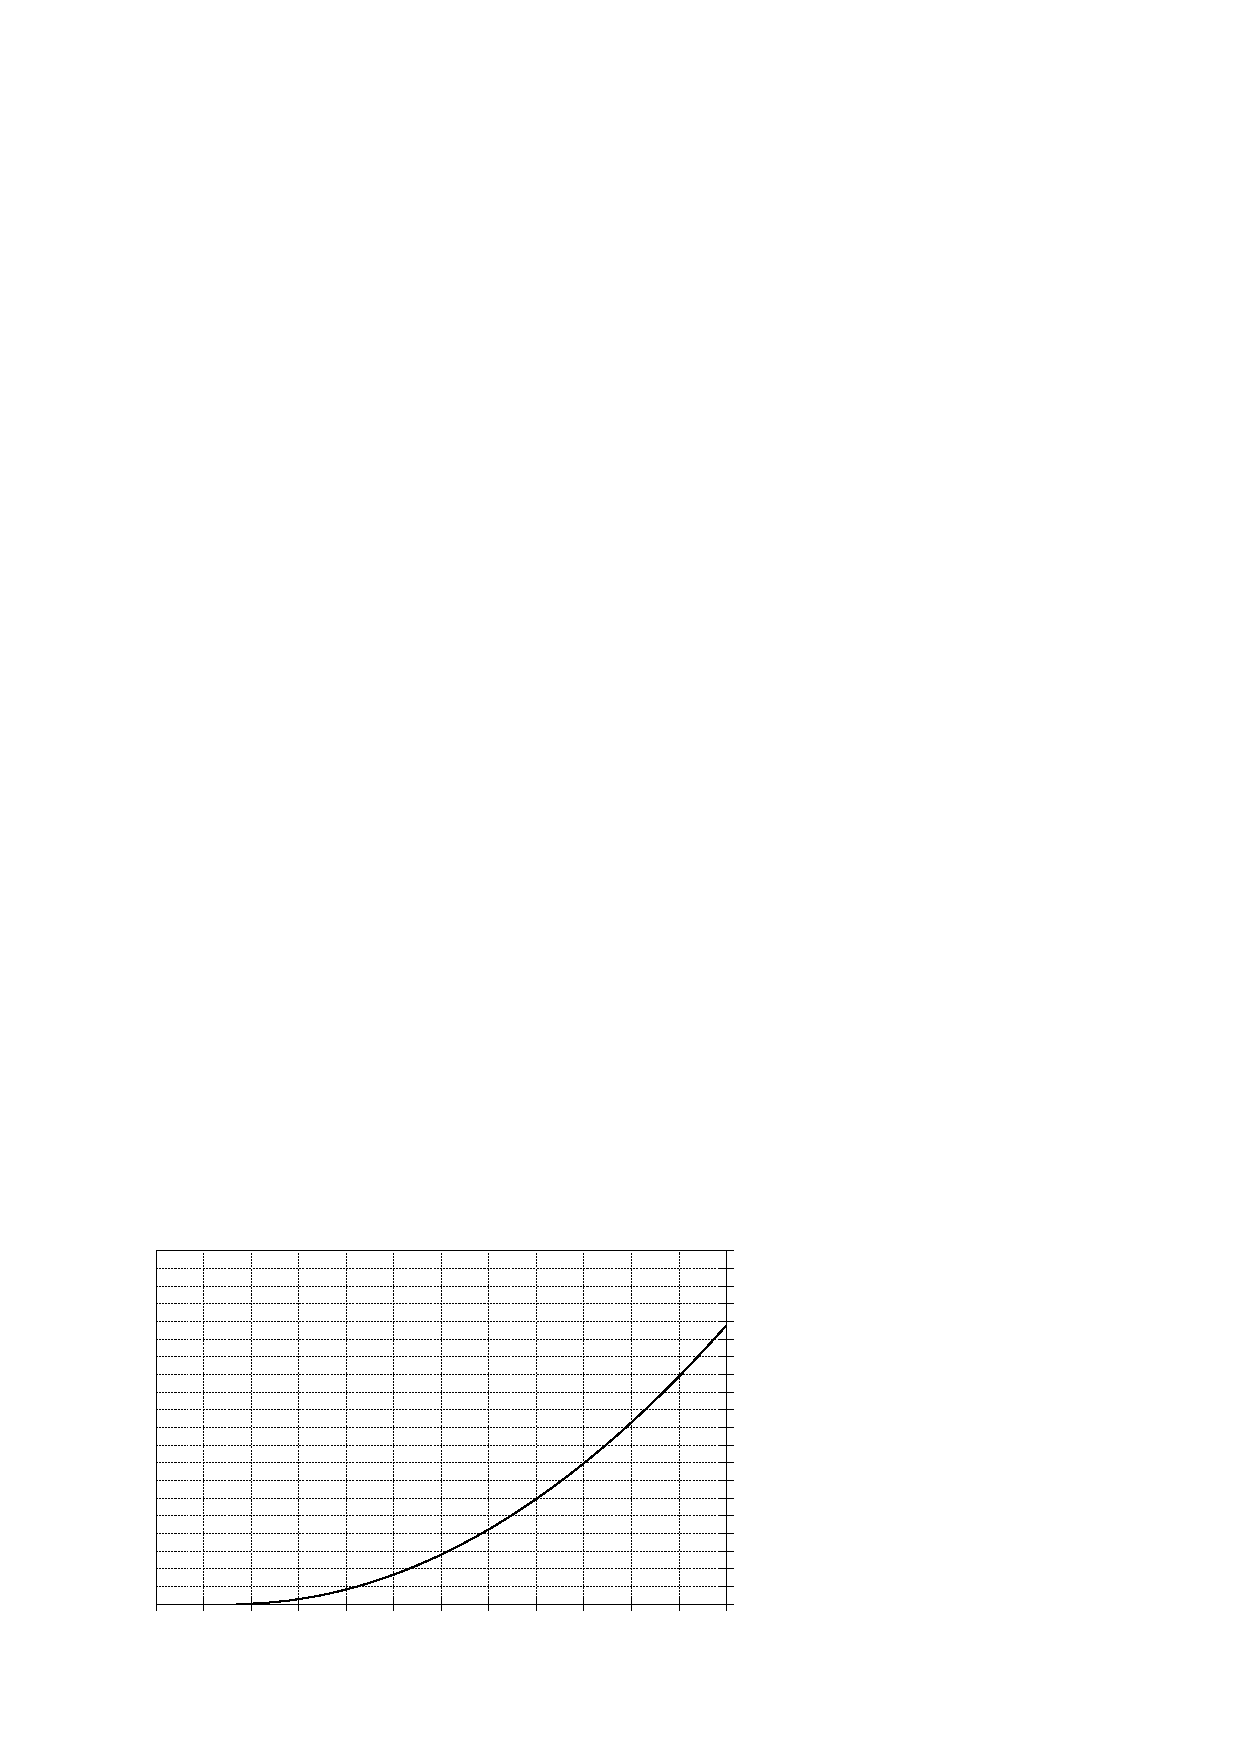
\includegraphics[width={316.80bp},height={201.50bp}]{curva1}}%
    \gplfronttext
  \end{picture}%
\endgroup

    \caption{Curvas características de los transistores JFET.}
    \label{curva01}
\end{figure}


%\section{Polarización en cd}

\subsection{BJT}
Un transistor debe ser apropiadamente polarizado con un voltaje de cd para que
opere como amplificador lineal. Se debe ajustar el punto de operación en cd de
modo que las variaciones de la señal en la terminal de entrada se amplifiquen y
reproduzcan con precisión en la terminal de salida. El punto de operación en cd
a menudo se conoce como \textbf{punto Q}.

Si un amplificador no se polariza con voltajes de cd correctos a la entrada y
salida, puede irse a saturación o a corte cuando se aplique una señal de
entrada.

La operación en cd de un circuito con un transistor se describe gráficamente con
una \textbf{recta de carga en cd}. Esta es una recta sobre las curvas
características desde el valor de saturación donde
$I_{\text{C}} = I_{\text{C(sat)}}$ sobre el eje $y$ hasta el valor de corte
donde $V_{\text{CE}} = V_{\text{CC}}$ sobre el eje $x$. El circuito externo
($V_{\text{CC}}$ y $R_{\text{C}}$) determina la recta de carga, no el transistor
mismo. El punto donde la recta de carga corta una curva característica
representa al punto Q con ese valor particular de $I_{\text{B}}$ \cite{Floyd}.

\subsubsection{Divisor de voltaje}
El método mas utilizado para la polarización del transistor es por medio de un
divisor de voltaje como se muestra en la \textbf{figura~\ref{figura11}}.

\begin{figure}[!ht]
\centering
\includegraphics[scale=0.26]{diagramas/figura11.eps}
\caption{Circuito divisor de voltaje.}
\label{figura11}
\end{figure}

Para el calculo de los valores del circuito se utilizan las siguientes
ecuaciones \cite{Boylestad}:
\begin{equation*}
    \begin{split}
        R_{\text{TH}} &= \frac{R_1\,R_2}{R_1+R_2}\\
        V_{\text{TH}} &= \frac{R_2}{R_1+R_2}\,V_{\text{CC}}\\
        I_{\text{B}}  &= \frac{V_{\text{TH}}-V_{\text{BE}}}
                         {R_{\text{TH}}+(\beta + 1)\,R_{\text{E}}}\\
        V_{\text{CE}} &= V_{\text{CC}} - I_{\text{C}}\,(R_C + R_E)\\
    \end{split}
\end{equation*}

\subsubsection{Criterios de diseño}
En general, los divisores de voltaje se diseñan de modo que la corriente en la
base sea mucho menor que la corriente ($I_{\text{2}}$) que pasa a través de
$R_{\text{2}}$, se dice que un divisor de voltaje en el que la corriente en la
base es pequeña, comparada con la corriente en $R_{\text{2}}$, es un
\textbf{divisor de voltaje rígido} porque el voltaje en la base es relativamente
independiente de los diferentes transistores y efectos de la temperatura
\cite{Floyd}.

Por tanto, para diseñar un divisor de voltaje rígido se debe cumplir la
siguiente ecuación:
\begin{equation*}
    \beta_{\text{CD}}\,R_{\text{E}} > 10\,R_{\text{2}}
\end{equation*}

La necesidad de incluir un resistor del emisor a tierra fue estabilizar la
polarización de cd de modo que el cambio de la corriente del colector provocado
por corrientes de fuga en el transistor y por la $\beta$ de éste, no provoquen
un gran desplazamiento del punto de operación. El resistor del emisor no puede
ser demasiado grande porque el voltaje a través de él limita el intervalo de
variación del voltaje del colector al emisor. Se recomienda que el voltaje de
emisor a tierra por lo general sea de alrededor de un cuarto a un décimo del
voltaje de alimentación \cite{Boylestad}.
\begin{equation*}
    \begin{split}
        V_{\text{E}} = \frac{1}{10}\,V_{\text{CC}}
    \end{split}
\end{equation*}

Por ultimo, al diseñar un amplificador con transistor se desea una salida con
máxima excursión no distorsionada. Si la señal de entrada en ca es simétrica
alrededor de cero, se puede obtener una excursión máxima colocando el punto $Q$
en el centro de la linea de carga \cite{Savant}.
\begin{equation*}
    V_{\text{CE}} = \frac{V_{\text{CC}}}{2}
\end{equation*}

\subsubsection{Voltaje de alimentación}
Para el diseño del amplificador se seleccionó un voltaje de alimentación de
$9\,[\text{V}]$.
\begin{equation*}
    V_{\text{CC}} = 9\,[\text{V}]
\end{equation*}

\subsubsection{Resistencias disponibles}
Se cuenta con una serie de resistencias de $0.5[\text{W}]$ con los valores
detallados en el \textbf{cuadro~\ref{cuadro06}}.

\begin{table}[!ht]
\begin{center}
    \begin{tabular}{|c|c|c|c|c|c|c|c|c|c|}
    \hline
    $1[\Omega]$ & $10[\Omega]$ & $22[\Omega]$ & $47[\Omega]$ & $100[\Omega]$ &
    $150[\Omega]$ & $200[\Omega]$ & $220[\Omega]$ & $270[\Omega]$ &
    $330[\Omega]$
    \tabularnewline \hline
    $470[\Omega]$ & $510[\Omega]$ & $680[\Omega]$ & $1[k{\Omega}]$ &
    $2[k{\Omega}]$ & $2.2[k{\Omega}]$ & $3.3[k{\Omega}]$ & $4.7[k{\Omega}]$ &
    $5.1[k{\Omega}]$ & $6.8[k{\Omega}]$
    \tabularnewline \hline
    $10[k{\Omega}]$ & $20[k{\Omega}]$ & $47[k{\Omega}]$ & $51[k{\Omega}]$ &
    $68[k{\Omega}]$ & $100[k{\Omega}]$ & $220[k{\Omega}]$ & $330[k{\Omega}]$ &
    $510[k{\Omega}]$ & $1[M{\Omega}]$
    \tabularnewline \hline
    \end{tabular}
\end{center}
\caption{Valores de resistencias disponibles para el diseño.}
\label{cuadro06}
\end{table}

\subsubsection{Calculo computarizado}
Una vez descritos los criterios de diseño y las formulas para el calculo de las
resistencias del divisor de voltaje, se ha escrito un programa para el software
matemático \emph{Octave}, que permute todas las combinaciones posibles de las 
resistencia e imprima aquellas que cumplen todos los criterios.

\scriptsize
\begin{shaded}
\begin{verbatim}
% polarizacion por divisor de voltaje (2N2222A NPN)
Vcc = 9;            % [V]
Vbe = 0.675;        % [V]
B = 302;

% resistencias disponibles
R = [
    1 ...
    10            22             47 ...
    100 150 200   220 270 330    470   510    680 ...
    1000    2000  2200    3300   4700  5100   6800 ...
    10000   20000                47000 51000  68000 ...
    100000        220000  330000       510000 ...
    1000000
];

count = 1;
printf('\tR1[Ω]\tR2[Ω]\tRc[Ω]\tRe[Ω]\t->\tVce[V]\tVe[V]\tIb[µA]\tIc[mA]\tP1[mW]\tP2[mW]\tPc[mW]\tPe[mW]\n');

for (h = 1:length(R))
    for (i = 1:length(R))
        for (j = 1:length(R))
            for (k = 1:length(R))
                R1 = R(h);
                R2 = R(i);
                Rc = R(j);
                Re = R(k);

                Rth = (R1 * R2) / (R1 + R2);
                Vth = ( R2 / (R1 + R2)) * Vcc;

                Ib = (Vth - Vbe) / (Rth + ( (B + 1) * Re) );
                Ic = B * Ib;
                Ie = Ic + Ib;
                Vce = Vcc - (Ic * (Rc + Re));
                Vc = Ic * Rc;
                Ve = Ie * Re;

                if(
                    (B * Re) > (10 * R2)&&          % divisor de voltaje rigido
                    (abs((Vcc / 2) - Vce) < 0.1)&&  % 4.4 < Vce < 4.6[V]
                    (abs((0.1 * Vcc) - Ve) < 0.1)&& % 0.8 < Ve < 1.0[V]
                    (Ic > 10e-3)                    % Ic > 10[mA]
                )
                    printf(
                        '%d\t%d\t%d\t%d\t%d\t->\t%.2f\t%.2f\t%.2f\t%.2f\t%.2f\t%.2f\t%.2f\t%.2f\n',
                        count,
                        R(h), R(i), R(j), R(k),
                        Vce,
                        Ve,
                        Ib * 1e6,
                        Ic * 1e3,
                        (((R1 / (R1 + R2)) * Vcc)^2 / R1) * 1e3,
                        (((R2 / (R1 + R2)) * Vcc)^2 / R2) * 1e3,
                        Ic^2 * Rc * 1e3,
                        Ve * Ie * 1e3
                    );

                    count++;
                endif
            endfor
        endfor
    endfor
endfor
\end{verbatim}
\end{shaded}
\normalsize

\subsubsection{Resultados del calculo computarizado}
La salida del programa detalla los valores de las cuatro resistencias ($R_1$,
$R_2$, $R_C$, $R_E$), el voltaje de colector-emisor ($V_{\text{CE}}$), el
voltaje de la resistencia emisor ($V_{\text{E}}$), la corriente de base ($I_B$)
y la corriente de colector ($I_C$), estos valores pueden verse en el
\textbf{cuadro~\ref{cuadro07}}.

\begin{table}[!h]
\begin{center}
    \begin{tabular}{|c|c|c|c||c|c||c|c|}
    \hline
    $R_1[\Omega]$ & $R_2[\Omega]$ & $R_C[\Omega]$ & $R_E[\Omega]$ &
    $V_{\text{CE}}[V]$ & $V_{\text{E}}[V]$ &
    $I_{\text{B}}[\mu{A}]$ & $I_{\text{C}}[mA]$
    \tabularnewline \hline \hline
    $  1k$ & $ 200$ & $100$ & $22$ & $4.55$ & $0.80$ & $120.74$ & $36.46$ \tabularnewline \hline
    $4.7k$ & $  1k$ & $200$ & $47$ & $4.52$ & $0.85$ & $ 60.00$ & $18.12$ \tabularnewline \hline
    \end{tabular}
\end{center}
\caption{Resultados del calculo computarizado.}
\label{cuadro07}
\end{table}

\subsubsection{Simulación de computadora}
Se utilizó el software \emph{Quite Universal Circuit Simulator.} versión 23.3.1
para simular el circuito, este puede verse en la
\textbf{figura~\ref{figura12}} y los valores calculados en el simulador pueden
verse en el \textbf{cuadro~\ref{cuadro08}}.

\begin{figure}[!h]
\centering
\includegraphics[scale=0.54]{diagramas/figura12.eps}
\caption{Simulación del circuito.}
\label{figura12}
\end{figure}

\begin{table}[!h]
\begin{center}
    \begin{tabular}{|c|c|c|c||c|c||c|c|}
    \hline
    $R_1[\Omega]$ & $R_2[\Omega]$ & $R_C[\Omega]$ & $R_E[\Omega]$ &
    $V_{\text{CE}}[V]$ & $V_{\text{E}}[V]$ &
    $I_{\text{C}}[\mu{A}]$ & $I_{\text{C}}[mA]$
    \tabularnewline \hline \hline
    $  1k$ & $200$ & $100$ & $22$ & $4.79$ & $0.762$ & $ 190$ & $34.5$ \tabularnewline \hline
    $4.7k$ & $ 1k$ & $200$ & $47$ & $4.71$ & $0.820$ & $93.9$ & $17.4$ \tabularnewline \hline
    \end{tabular}
\end{center}
\caption{Resultados obtenidos de la simulación.}
\label{cuadro08}
\end{table}

\subsubsection{Placa de prueba}
El circuito armado puede verse en la \textbf{figura~\ref{figura13}}, alimentado
por una fuente estable de $9[\text{V}]$.

En el circuito se fueron variando las resistencias obtenidas en el calculo
anterior, y se midieron los valores de voltaje y corriente, estos se muestran
en el \textbf{cuadro~\ref{cuadro09}}.

\begin{figure}[!h]
\centering
\includegraphics[scale=0.10]{diagramas/figura13.eps}
\caption{Polarización con divisor de voltaje en placa de pruebas.}
\label{figura13}
\end{figure}

\begin{table}[!h]
\begin{center}
    \begin{tabular}{|c|c|c|c||c|c||c|c|}
    \hline
    $R_1[\Omega]$ & $R_2[\Omega]$ & $R_C[\Omega]$ & $R_E[\Omega]$ &
    $V_{\text{CE}}[V]$ & $V_{\text{E}}[V]$ &
    $I_{\text{B}}[\mu{A}]$ & $I_{\text{C}}[mA]$
    \tabularnewline \hline \hline
    $ 1k$ & $ 200$ & $100$ & $22$ & $4.63$ & $0.805$ & $125.6$ & $36.6$ \tabularnewline \hline
    $10k$ & $3.3k$ & $ 47$ & $10$ & $3.01$ & $1.165$ & $ 0.03$ & $24.7$ \tabularnewline \hline
    \end{tabular}
\end{center}
\caption{Valores medidos en la placa de pruebas.}
\label{cuadro09}
\end{table}

\subsubsection{Valores de polarización}
Puede observarse que en la segunda medición los valores entre el calculo
teórico, simulación y medición real hay muchas discrepancias, por lo que se
utilizaran los valores de la primera medición. Con lo cual se halla el punto $Q$
de operación, que puede verse en la \textbf{figura~\ref{curva02}}.

\begin{figure}[!ht]
    \centering
    % GNUPLOT: LaTeX picture with Postscript
\begingroup
  \makeatletter
  \providecommand\color[2][]{%
    \GenericError{(gnuplot) \space\space\space\@spaces}{%
      Package color not loaded in conjunction with
      terminal option `colourtext'%
    }{See the gnuplot documentation for explanation.%
    }{Either use 'blacktext' in gnuplot or load the package
      color.sty in LaTeX.}%
    \renewcommand\color[2][]{}%
  }%
  \providecommand\includegraphics[2][]{%
    \GenericError{(gnuplot) \space\space\space\@spaces}{%
      Package graphicx or graphics not loaded%
    }{See the gnuplot documentation for explanation.%
    }{The gnuplot epslatex terminal needs graphicx.sty or graphics.sty.}%
    \renewcommand\includegraphics[2][]{}%
  }%
  \providecommand\rotatebox[2]{#2}%
  \@ifundefined{ifGPcolor}{%
    \newif\ifGPcolor
    \GPcolorfalse
  }{}%
  \@ifundefined{ifGPblacktext}{%
    \newif\ifGPblacktext
    \GPblacktexttrue
  }{}%
  % define a \g@addto@macro without @ in the name:
  \let\gplgaddtomacro\g@addto@macro
  % define empty templates for all commands taking text:
  \gdef\gplbacktext{}%
  \gdef\gplfronttext{}%
  \makeatother
  \ifGPblacktext
    % no textcolor at all
    \def\colorrgb#1{}%
    \def\colorgray#1{}%
  \else
    % gray or color?
    \ifGPcolor
      \def\colorrgb#1{\color[rgb]{#1}}%
      \def\colorgray#1{\color[gray]{#1}}%
      \expandafter\def\csname LTw\endcsname{\color{white}}%
      \expandafter\def\csname LTb\endcsname{\color{black}}%
      \expandafter\def\csname LTa\endcsname{\color{black}}%
      \expandafter\def\csname LT0\endcsname{\color[rgb]{1,0,0}}%
      \expandafter\def\csname LT1\endcsname{\color[rgb]{0,1,0}}%
      \expandafter\def\csname LT2\endcsname{\color[rgb]{0,0,1}}%
      \expandafter\def\csname LT3\endcsname{\color[rgb]{1,0,1}}%
      \expandafter\def\csname LT4\endcsname{\color[rgb]{0,1,1}}%
      \expandafter\def\csname LT5\endcsname{\color[rgb]{1,1,0}}%
      \expandafter\def\csname LT6\endcsname{\color[rgb]{0,0,0}}%
      \expandafter\def\csname LT7\endcsname{\color[rgb]{1,0.3,0}}%
      \expandafter\def\csname LT8\endcsname{\color[rgb]{0.5,0.5,0.5}}%
    \else
      % gray
      \def\colorrgb#1{\color{black}}%
      \def\colorgray#1{\color[gray]{#1}}%
      \expandafter\def\csname LTw\endcsname{\color{white}}%
      \expandafter\def\csname LTb\endcsname{\color{black}}%
      \expandafter\def\csname LTa\endcsname{\color{black}}%
      \expandafter\def\csname LT0\endcsname{\color{black}}%
      \expandafter\def\csname LT1\endcsname{\color{black}}%
      \expandafter\def\csname LT2\endcsname{\color{black}}%
      \expandafter\def\csname LT3\endcsname{\color{black}}%
      \expandafter\def\csname LT4\endcsname{\color{black}}%
      \expandafter\def\csname LT5\endcsname{\color{black}}%
      \expandafter\def\csname LT6\endcsname{\color{black}}%
      \expandafter\def\csname LT7\endcsname{\color{black}}%
      \expandafter\def\csname LT8\endcsname{\color{black}}%
    \fi
  \fi
    \setlength{\unitlength}{0.0500bp}%
    \ifx\gptboxheight\undefined%
      \newlength{\gptboxheight}%
      \newlength{\gptboxwidth}%
      \newsavebox{\gptboxtext}%
    \fi%
    \setlength{\fboxrule}{0.5pt}%
    \setlength{\fboxsep}{1pt}%
    \definecolor{tbcol}{rgb}{1,1,1}%
\begin{picture}(5760.00,3600.00)%
    \gplgaddtomacro\gplbacktext{%
      \csname LTb\endcsname%%
      \put(380,440){\makebox(0,0)[r]{\strut{}}}%
      \put(380,736){\makebox(0,0)[r]{\strut{}}}%
      \put(380,1032){\makebox(0,0)[r]{\strut{}}}%
      \put(380,1328){\makebox(0,0)[r]{\strut{}}}%
      \put(380,1624){\makebox(0,0)[r]{\strut{}}}%
      \put(380,1920){\makebox(0,0)[r]{\strut{}}}%
      \put(380,2215){\makebox(0,0)[r]{\strut{}}}%
      \put(380,2511){\makebox(0,0)[r]{\strut{}}}%
      \put(380,2807){\makebox(0,0)[r]{\strut{}}}%
      \put(380,3103){\makebox(0,0)[r]{\strut{}}}%
      \put(380,3399){\makebox(0,0)[r]{\strut{}}}%
      \put(500,240){\makebox(0,0){\strut{}}}%
      \put(1044,240){\makebox(0,0){\strut{}}}%
      \put(1589,240){\makebox(0,0){\strut{}}}%
      \put(2133,240){\makebox(0,0){\strut{}}}%
      \put(2677,240){\makebox(0,0){\strut{}}}%
      \put(3222,240){\makebox(0,0){\strut{}}}%
      \put(3766,240){\makebox(0,0){\strut{}}}%
      \put(4310,240){\makebox(0,0){\strut{}}}%
      \put(4855,240){\makebox(0,0){\strut{}}}%
      \put(5399,240){\makebox(0,0){\strut{}}}%
      \csname LTb\endcsname%%
      \put(5508,1523){\makebox(0,0)[l]{\strut{}$I_{\text{B}} = 125.6[\mu{A}]$}}%
      \put(5508,2623){\makebox(0,0)[l]{\strut{}$I_{\text{B}} = 244.2[\mu{A}]$}}%
      \put(935,3251){\makebox(0,0)[l]{\strut{}$0.675[V]$}}%
      \put(3113,3251){\makebox(0,0)[l]{\strut{}$4.63[V]$}}%
      \put(5508,3251){\makebox(0,0)[l]{\strut{}$9[V]$}}%
    }%
    \gplgaddtomacro\gplfronttext{%
      \csname LTb\endcsname%%
      \put(190,1919){\rotatebox{-270.00}{\makebox(0,0){\strut{}$I_{\text{C}}[mA]$}}}%
      \put(2949,140){\makebox(0,0){\strut{}$V_{\text{CE}}[V]$}}%
    }%
    \gplgaddtomacro\gplbacktext{%
      \csname LTb\endcsname%%
      \put(380,440){\makebox(0,0)[r]{\strut{}}}%
      \put(380,736){\makebox(0,0)[r]{\strut{}}}%
      \put(380,1032){\makebox(0,0)[r]{\strut{}}}%
      \put(380,1328){\makebox(0,0)[r]{\strut{}}}%
      \put(380,1624){\makebox(0,0)[r]{\strut{}}}%
      \put(380,1920){\makebox(0,0)[r]{\strut{}}}%
      \put(380,2215){\makebox(0,0)[r]{\strut{}}}%
      \put(380,2511){\makebox(0,0)[r]{\strut{}}}%
      \put(380,2807){\makebox(0,0)[r]{\strut{}}}%
      \put(380,3103){\makebox(0,0)[r]{\strut{}}}%
      \put(380,3399){\makebox(0,0)[r]{\strut{}}}%
      \put(500,240){\makebox(0,0){\strut{}}}%
      \put(1044,240){\makebox(0,0){\strut{}}}%
      \put(1589,240){\makebox(0,0){\strut{}}}%
      \put(2133,240){\makebox(0,0){\strut{}}}%
      \put(2677,240){\makebox(0,0){\strut{}}}%
      \put(3222,240){\makebox(0,0){\strut{}}}%
      \put(3766,240){\makebox(0,0){\strut{}}}%
      \put(4310,240){\makebox(0,0){\strut{}}}%
      \put(4855,240){\makebox(0,0){\strut{}}}%
      \put(5399,240){\makebox(0,0){\strut{}}}%
      \csname LTb\endcsname%%
      \put(5508,1523){\makebox(0,0)[l]{\strut{}$I_{\text{B}} = 125.6[\mu{A}]$}}%
      \put(5508,2623){\makebox(0,0)[l]{\strut{}$I_{\text{B}} = 244.2[\mu{A}]$}}%
      \put(935,3251){\makebox(0,0)[l]{\strut{}$0.675[V]$}}%
      \put(3113,3251){\makebox(0,0)[l]{\strut{}$4.63[V]$}}%
      \put(5508,3251){\makebox(0,0)[l]{\strut{}$9[V]$}}%
    }%
    \gplgaddtomacro\gplfronttext{%
      \csname LTb\endcsname%%
      \put(190,1919){\rotatebox{-270.00}{\makebox(0,0){\strut{}$I_{\text{C}}[mA]$}}}%
      \put(2949,140){\makebox(0,0){\strut{}$V_{\text{CE}}[V]$}}%
    }%
    \gplbacktext
    \put(0,0){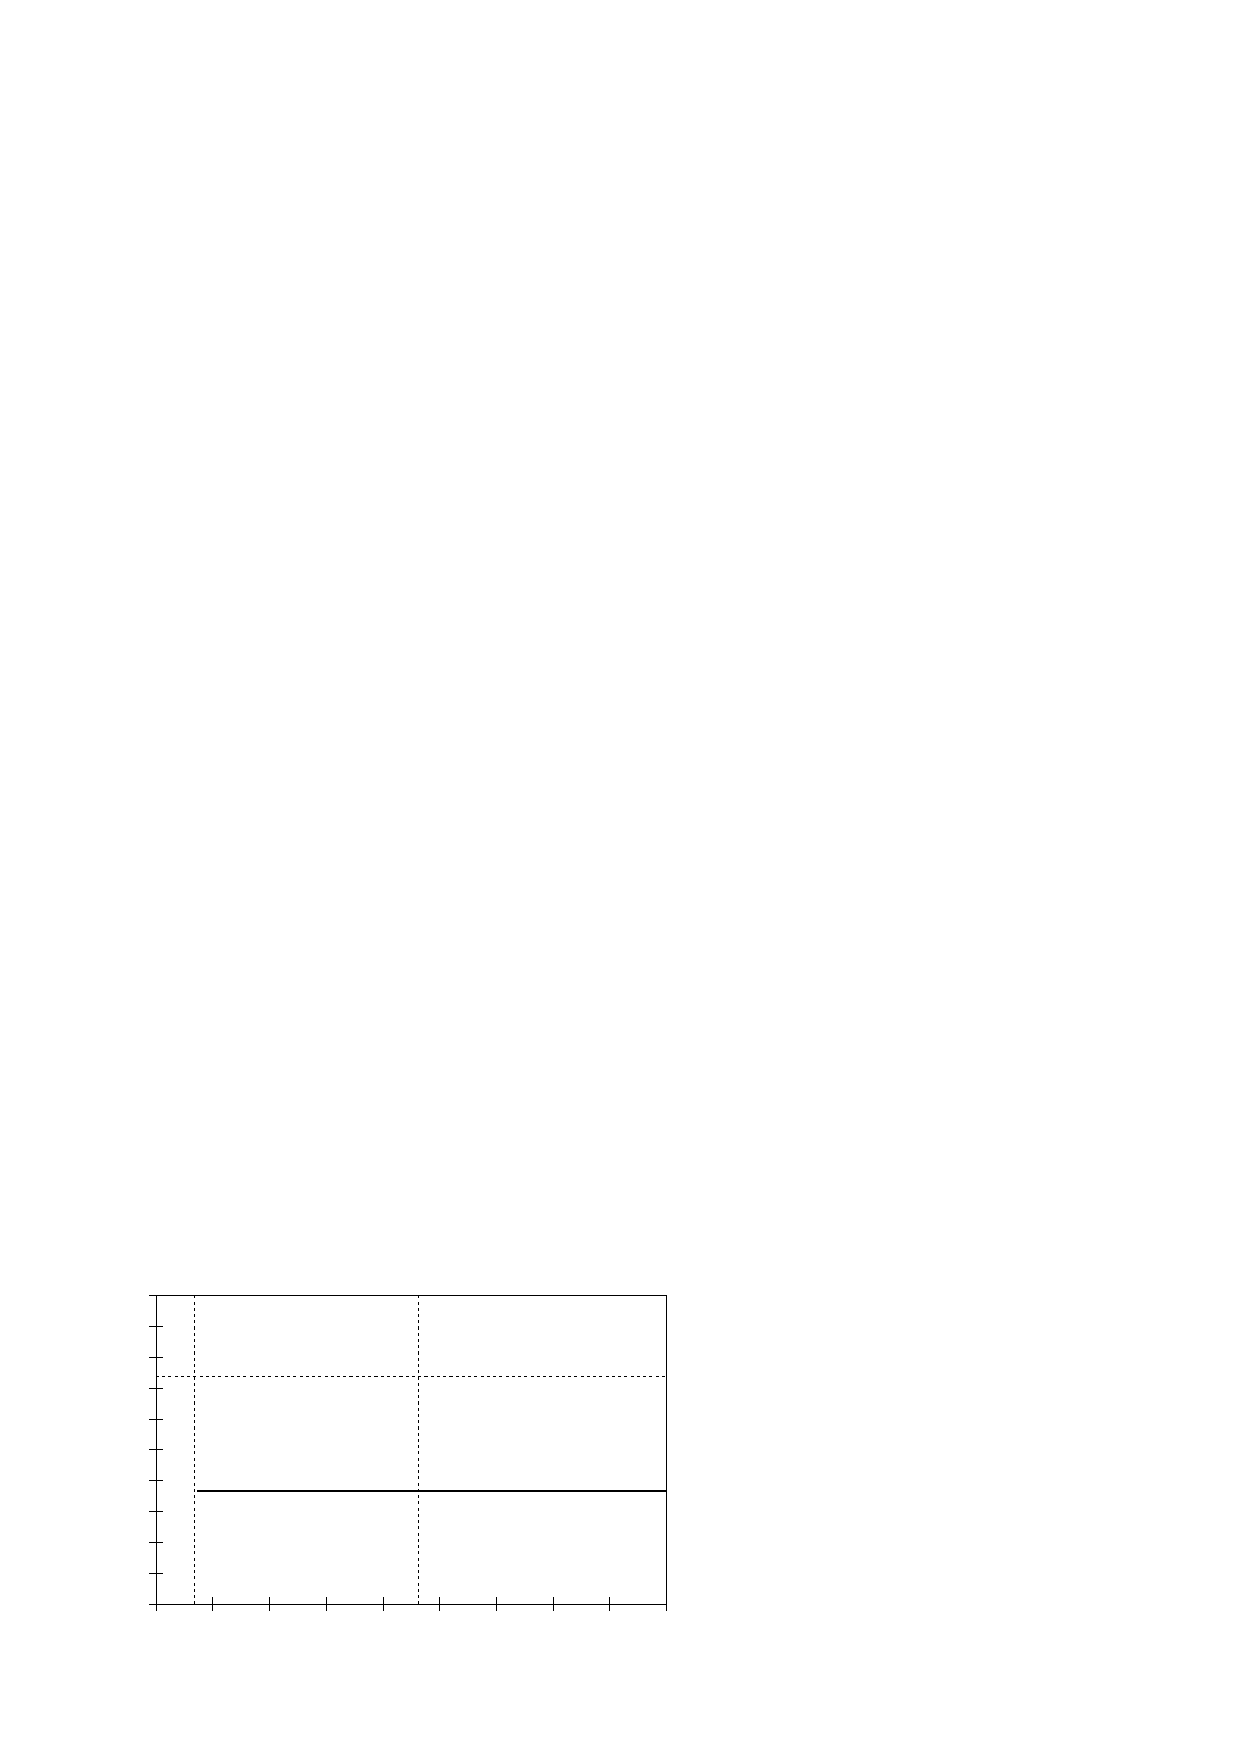
\includegraphics[width={288.00bp},height={180.00bp}]{curva2}}%
    \gplfronttext
  \end{picture}%
\endgroup

    \caption{Punto $Q$ hallado.}
    \label{curva02}
\end{figure}

Según las pruebas realizadas los valores obtenidos son:
\begin{equation*}
    \begin{split}
        R_{\text{1}} &= 1[k\Omega]\\
        R_{\text{2}} &= 200[\Omega]\\
        R_{\text{C}} &= 100[\Omega]\\
        R_{\text{E}} &= 22[\Omega]\\
\end{split}
\end{equation*}

Ecuación de la recta de carga:
\begin{equation*}
    I_{\text{C}} = \frac{9}{122} - \frac{1}{122}V_{\text{CE}}
\end{equation*}

Punto $Q$:
\begin{equation*}
    \begin{split}
        V_{\text{CE}} = 4.63\,[\text{V}]\\
        I_{\text{C}} = 36.6\,[\text{mA}]\\
    \end{split}
\end{equation*}

Rango máximo de corriente de base:
$-107.34[\mu{\text{A}}] < I_{\text{B}} < 107.34[\mu{\text{A}}]$.


%\subsection{FET}
Al igual que con el BJT, el propósito de la polarización es seleccionar el
voltaje de cd de compuerta a fuente apropiado para establecer un valor deseado
de la corriente en el drenaje y, por consiguiente, un punto Q apropiado
\cite{Floyd}.

\subsubsection{Divisor de voltaje}
La configuración del divisor de voltaje aplicada a amplificadores con
transistores BJT también se aplica a amplificadores con FET como se muestra en
la \textbf{figura~\ref{figura14}}. La construcción básica es exactamente la misma,
pero el análisis de cada una es muy diferente.

\begin{figure}[!ht]
\centering
\includegraphics[scale=0.26]{diagramas/figura14.eps}
\caption{Circuito divisor de voltaje.}
\label{figura14}
\end{figure}

Una curva de transferencia para un \textbf{JFET} se expresa aproximadamente
como:
\begin{equation*}
    I_{\text{D}} \cong I_{\text{DSS}}
    \left(1-\frac{V_{\text{GS}}}{V_{\text{GS(corte)}}}\right)^2
\end{equation*}

La recta de carga de CD con divisor de voltaje se determina de la siguiente
manera:

Con $I_\text{D} = 0$:
\begin{equation*}
    \begin{split}
        V_\text{S} &= I_{\text{D}}\,R_{\text{S}}
                   = (0)\,R_{\text{S}}
                   = 0[V]\\
        V_\text{GS} &= V_{\text{G}} - V_{\text{S}}
                    = V_{\text{G}} - 0[V]
                    = V_{\text{G}}\\
    \end{split}
\end{equation*}

Donde $V_{\text{G}}$:
\begin{equation*}
    V_{\text{G}} = \left(\frac{R_2}{R_1+R_2}\right)\,V_{\text{DD}}
\end{equation*}

Por consiguiente, un punto sobre la recta está en $I_{\text{D}} = 0$ y
$V_{\text{GS}} = V_{\text{G}}$.

Con $V_{\text{GS}} = 0$:
\begin{equation*}
    I_\text{D} = \frac{V_{\text{G}} - V_{\text{GS}}}{R_{\text{S}}}
               = \frac{V_{\text{G}}}{R_{\text{S}}}
\end{equation*}

El punto donde la recta de carga corta la curva de transferencia es el punto
$Q$ \cite{Floyd}.
\begin{equation*}
    \left(\frac{I_{\text{DSS}}}{V_{\text{GS(corte)}}^2}\right)\,
    V_{\text{GS}}^2 + \left(\frac{1}{R_{\text{S}}}-
    \frac{2\,I_{\text{DSS}}}{V_{\text{GS(corte)}}}\right)\,
    V_{\text{GS}}+
    \left(I_{\text{DSS}}-\frac{V_{\text{G}}}{R_{\text{S}}}\right) = 0
\end{equation*}

Resolviendo la ecuación cuadrática es posible encontrar el punto $Q$ del
circuito.

\subsubsection{Criterios de diseño}
Normalmente es deseable polarizar un JFET cerca del punto medio de su curva de
transferencia donde $I_{\text{D}} = I_{\text{DSS}}/2$. En condiciones de señal,
la polarización en el punto medio permite que la cantidad máxima de corriente en
el drenaje oscile entre $I_{\text{DSS}}$ y $0$ \cite{Floyd}.
\begin{equation*}
    \begin{split}
        I_{\text{D}} &\rightarrow 0.5\,I_{\text{DSS}}\\
        V_{\text{G}} &\rightarrow 0.5\,V_{\text{GS(corte)}}\\
    \end{split}
\end{equation*}

De la misma manera que en la polarización BJT, también se considerará que el
voltaje entre el drenaje y fuente se encuentre en el punto medio del voltaje de
alimentación:
\begin{equation*}
    V_{\text{GS}} = \frac{1}{2}\,V_{\text{DD}}
\end{equation*}

Nótese que no se necesita colocar el punto Q en el centro de la linea de carga
de ca como se hizo para la polarización del BJT; esto se debe a que normalmente
se utiliza un amplificador FET en la entrada del amplificador para sacar ventaja
de la alta resistencia de entrada. En este punto, los niveles de tensión son tan
pequeños que no se excita al amplificador con grades excursiones. Además, como
las curvas características no son lineales, se produciría distorsión con grandes
excursiones de entrada \cite{Savant}.

Se considerara usar el conjunto de valores cuyo $V_{\text{DS}}$ sea el mas alto
posible:
\begin{equation*}
    V_{\text{DS}} = V_{\text{DD}} - I_{\text{D}}\,(R_{\text{D}} + R_{\text{S}})
\end{equation*}

También se deben considerar las potencias disipadas máximas por las
resistencias:
\begin{equation*}
    \{P_{R_1}, P_{R_2}, P_{R_D}, P_{R_S}\} < 0.2[\text{W}]\\
\end{equation*}

\subsubsection{Voltaje de alimentación}
Para el diseño del amplificador se seleccionó un voltaje de alimentación de
$9\,[\text{V}]$.
\begin{equation*}
    V_{\text{CC}} = 9\,[\text{V}]
\end{equation*}

\subsubsection{Resistencias disponibles}
Se cuenta con una serie de resistencias de $0.5[\text{W}]$ con los valores
detallados en el \textbf{cuadro~\ref{cuadro06}}.

\subsubsection{Calculo computarizado}
Una vez descritos los criterios de diseño y las formulas para el calculo de las
resistencias del divisor de voltaje, se ha escrito un programa para el software
matemático \emph{Octave}, que permute todas las combinaciones posibles de las 
resistencia e imprima aquellas que cumplen todos los criterios.

\scriptsize
\begin{shaded}
\begin{verbatim}
% polarizacion por divisor de voltaje (2N3819 canal n)
Vdd = 9;            % [V]
Idss = 15.8e-3;     % [A]
Vgso = -1.037;      % [V]

% resistencias disponibles
R = [
    1 ...
    10            22             47 ...
    100 150 200   220 270 330    470   510    680 ...
    1000    2000  2200    3300   4700  5100   6800 ...
    10000   20000                47000 51000  68000 ...
    100000        220000  330000       510000 ...
    1000000
];

count = 1;
printf(' ,R1[Ω],R2[Ω],Rd[Ω],Rs[Ω] -> Vg[V]\t\tId[mA] Vds[V],P1[mW],P2[mW],Pd[mW],Ps[mW]\n');

for (h = 1:length(R))
    for (i = 1:length(R))
        for (j = 1:length(R))
            for (k = 1:length(R))
                R1 = R(h);
                R2 = R(i);
                Rd = R(j);
                Rs = R(k);

                Vg = (R2 / (R1 + R2)) * Vdd;    % Id = 0
                Id = Vg / Rs;                   % Vgs = 0

                QVg = roots([Idss/(Vgso^2), (1/Rs) - (2*(Idss/Vgso)), Idss-Id]);
                QId = (-1/Rs) * (QVg(2) - Vg);

                P1 = ((Vdd - QVg(2))^2) / R1;
                P2 = (QVg(2)^2) / R2;
                Pd = QId^2 * Rd;
                Ps = QId^2 * Rs;

                Vds = Vdd - (QId * (Rd + Rs));

                if(
                    (abs(Vgso - (2 * QVg(2))) < 0.4)&&         % Vg -> Vgs0/2
                    (abs(Idss - (2 * QId)) < 0.00075)&&     % Id -> Idss/2
                    (abs((Vdd / 2) - Vds) < 0.5)&&          % 4.0 < Vds < 5.0[V]
                    (0.001<P1)&&(P1<0.2)&&                  % 0.001 < P1 < 0.2
                    (0.001<P2)&&(P2<0.2)&&                  % 0.001 < P2 < 0.2
                    (0.001<Pd)&&(Pd<0.2)&&                  % 0.001 < Pd < 0.2
                    (0.001<Ps)&&(Ps<0.2)                    % 0.001 < Ps < 0.2
                )
                    printf(
                        '%d,%d,%d,%d,%d -> (%.2f, 0) (0, %.3f) %.2f,%.2f,%.2f,%.2f,%.2f,%.2f,%.2f\n',
                        count,
                        R(h), R(i), R(j), R(k),
                        Vg,Id * 1e3,
                        QVg(2), QId * 1e3,
                        Vds,
                        P1 * 1e3,
                        P2 * 1e3,
                        Pd * 1e3,
                        Ps * 1e3
                    );

                    count++;
                endif
            endfor
        endfor
    endfor
endfor
\end{verbatim}
\end{shaded}
\normalsize

\subsubsection{Resultados del calculo computarizado}
La salida del programa detalla los valores de las cuatro resistencias ($R_1$,
$R_2$, $R_D$, $R_S$), los valores de potencia en cada una de las resistencias
($P_1$, $P_2$, $P_D$, $P_S$), estos valores pueden verse en el
\textbf{cuadro~\ref{cuadro10}}.

\begin{table}[!h]
\begin{center}
    \begin{tabular}{|c|c|c|c||c||c|c|c|c|}
    \hline
    $R_1[\Omega]$ & $R_2[\Omega]$ & $R_D[\Omega]$ & $R_S[\Omega]$ &
    $V_{DS}[V]$ &
    $P_1[mW]$ & $P_2[mW]$ & $P_D[mW]$ & $P_S[mW]$
    \tabularnewline \hline \hline
    $ 470$ & $ 47$ & $470$ & $150$ & $4.30$ & $184.76$ & $2.16$ & $27.0$ & $8.62$ \tabularnewline \hline
    $1000$ & $100$ & $470$ & $150$ & $4.30$ & $ 86.84$ & $1.02$ & $27.0$ & $8.62$ \tabularnewline \hline
    \end{tabular}
\end{center}
\caption{Resultados del calculo computarizado.}
\label{cuadro10}
\end{table}

Mientras que los valores de voltaje de compuerta ($V_{\text{G}}$) y la corriente
de drenaje ($I_D$) son fijos para todos los casos.
\begin{equation*}
    \begin{split}
        V_{\text{G}} &= -0.32[V]\\
        I_{\text{D}} &= 7.58[mA]\\
    \end{split}
\end{equation*}

\subsubsection{Simulación de computadora}
Se utilizó el software \emph{Quite Universal Circuit Simulator.} versión 23.3.1
para simular el circuito, este puede verse en la
\textbf{figura~\ref{figura15}} y los valores calculados en el simulador pueden
verse en el \textbf{cuadro~\ref{cuadro11}}.

\begin{figure}[!h]
\centering
\includegraphics[scale=1.00]{diagramas/figura15.eps}
\caption{Simulación del circuito.}
\label{figura15}
\end{figure}

\begin{table}[!h]
\begin{center}
    \begin{tabular}{|c|c|c|c||c||c|c|}
    \hline
    $R_1[\Omega]$ & $R_2[\Omega]$ & $R_D[\Omega]$ & $R_S[\Omega]$ &
    $V_{\text{DS}}$ & $V_{\text{G}}[V]$ & $I_{\text{D}}[mA]$
    \tabularnewline \hline \hline
    $ 470$ & $ 47$ & $470$ & $150$ & $4.11$ & $-0.364$ & $7.88$ \tabularnewline \hline
    $1000$ & $100$ & $470$ & $150$ & $4.11$ & $-0.364$ & $7.88$ \tabularnewline \hline
    \end{tabular}
\end{center}
\caption{Resultados obtenidos de la simulación.}
\label{cuadro11}
\end{table}

\subsubsection{Placa de prueba}
El circuito armado puede verse en la \textbf{figura~\ref{figura16}}, alimentado
por una fuente estable de $9[\text{V}]$.

En el circuito se fueron variando las resistencias obtenidas en el calculo
anterior, y se midieron los valores de voltaje y corriente, estos se muestran
en el \textbf{cuadro~\ref{cuadro12}}.

\begin{figure}[!h]
\centering
\includegraphics[scale=0.125]{diagramas/figura16.eps}
\caption{Polarización con divisor de voltaje en placa de pruebas.}
\label{figura16}
\end{figure}

\begin{table}[!h]
\begin{center}
    \begin{tabular}{|c|c|c|c||c||c|c|}
    \hline
    $R_1[\Omega]$ & $R_2[\Omega]$ & $R_D[\Omega]$ & $R_S[\Omega]$ &
    $V_{\text{DS}}$ & $V_{\text{G}}[V]$ & $I_{\text{D}}[mA]$
    \tabularnewline \hline \hline
    $ 470$ & $ 47$ & $470$ & $150$ & $4.62$ & $-0.208$ & $7.03$ \tabularnewline \hline
    $1000$ & $100$ & $470$ & $150$ & $4.65$ & $-0.209$ & $7.00$ \tabularnewline \hline
    \end{tabular}
\end{center}
\caption{Valores medidos en la placa de pruebas.}
\label{cuadro12}
\end{table}

\subsubsection{Valores de polarización}
Considerando que todos los valores obtenidos tienen valores similares, se
utilizaran los de menor disipación de potencia. Con lo cual se halla el punto
$Q$ de operación, que puede verse en la \textbf{figura~\ref{curva03}}.

\begin{figure}[!ht]
    \centering
    % GNUPLOT: LaTeX picture with Postscript
\begingroup
  \makeatletter
  \providecommand\color[2][]{%
    \GenericError{(gnuplot) \space\space\space\@spaces}{%
      Package color not loaded in conjunction with
      terminal option `colourtext'%
    }{See the gnuplot documentation for explanation.%
    }{Either use 'blacktext' in gnuplot or load the package
      color.sty in LaTeX.}%
    \renewcommand\color[2][]{}%
  }%
  \providecommand\includegraphics[2][]{%
    \GenericError{(gnuplot) \space\space\space\@spaces}{%
      Package graphicx or graphics not loaded%
    }{See the gnuplot documentation for explanation.%
    }{The gnuplot epslatex terminal needs graphicx.sty or graphics.sty.}%
    \renewcommand\includegraphics[2][]{}%
  }%
  \providecommand\rotatebox[2]{#2}%
  \@ifundefined{ifGPcolor}{%
    \newif\ifGPcolor
    \GPcolorfalse
  }{}%
  \@ifundefined{ifGPblacktext}{%
    \newif\ifGPblacktext
    \GPblacktexttrue
  }{}%
  % define a \g@addto@macro without @ in the name:
  \let\gplgaddtomacro\g@addto@macro
  % define empty templates for all commands taking text:
  \gdef\gplbacktext{}%
  \gdef\gplfronttext{}%
  \makeatother
  \ifGPblacktext
    % no textcolor at all
    \def\colorrgb#1{}%
    \def\colorgray#1{}%
  \else
    % gray or color?
    \ifGPcolor
      \def\colorrgb#1{\color[rgb]{#1}}%
      \def\colorgray#1{\color[gray]{#1}}%
      \expandafter\def\csname LTw\endcsname{\color{white}}%
      \expandafter\def\csname LTb\endcsname{\color{black}}%
      \expandafter\def\csname LTa\endcsname{\color{black}}%
      \expandafter\def\csname LT0\endcsname{\color[rgb]{1,0,0}}%
      \expandafter\def\csname LT1\endcsname{\color[rgb]{0,1,0}}%
      \expandafter\def\csname LT2\endcsname{\color[rgb]{0,0,1}}%
      \expandafter\def\csname LT3\endcsname{\color[rgb]{1,0,1}}%
      \expandafter\def\csname LT4\endcsname{\color[rgb]{0,1,1}}%
      \expandafter\def\csname LT5\endcsname{\color[rgb]{1,1,0}}%
      \expandafter\def\csname LT6\endcsname{\color[rgb]{0,0,0}}%
      \expandafter\def\csname LT7\endcsname{\color[rgb]{1,0.3,0}}%
      \expandafter\def\csname LT8\endcsname{\color[rgb]{0.5,0.5,0.5}}%
    \else
      % gray
      \def\colorrgb#1{\color{black}}%
      \def\colorgray#1{\color[gray]{#1}}%
      \expandafter\def\csname LTw\endcsname{\color{white}}%
      \expandafter\def\csname LTb\endcsname{\color{black}}%
      \expandafter\def\csname LTa\endcsname{\color{black}}%
      \expandafter\def\csname LT0\endcsname{\color{black}}%
      \expandafter\def\csname LT1\endcsname{\color{black}}%
      \expandafter\def\csname LT2\endcsname{\color{black}}%
      \expandafter\def\csname LT3\endcsname{\color{black}}%
      \expandafter\def\csname LT4\endcsname{\color{black}}%
      \expandafter\def\csname LT5\endcsname{\color{black}}%
      \expandafter\def\csname LT6\endcsname{\color{black}}%
      \expandafter\def\csname LT7\endcsname{\color{black}}%
      \expandafter\def\csname LT8\endcsname{\color{black}}%
    \fi
  \fi
    \setlength{\unitlength}{0.0500bp}%
    \ifx\gptboxheight\undefined%
      \newlength{\gptboxheight}%
      \newlength{\gptboxwidth}%
      \newsavebox{\gptboxtext}%
    \fi%
    \setlength{\fboxrule}{0.5pt}%
    \setlength{\fboxsep}{1pt}%
    \definecolor{tbcol}{rgb}{1,1,1}%
\begin{picture}(6480.00,4030.00)%
    \gplgaddtomacro\gplbacktext{%
      \csname LTb\endcsname%%
      \put(3190,440){\makebox(0,0)[r]{\strut{}}}%
      \csname LTb\endcsname%%
      \put(3190,864){\makebox(0,0)[r]{\strut{}}}%
      \csname LTb\endcsname%%
      \put(3190,1287){\makebox(0,0)[r]{\strut{}}}%
      \csname LTb\endcsname%%
      \put(3190,1711){\makebox(0,0)[r]{\strut{}}}%
      \csname LTb\endcsname%%
      \put(3190,2135){\makebox(0,0)[r]{\strut{}}}%
      \csname LTb\endcsname%%
      \put(3190,2558){\makebox(0,0)[r]{\strut{}}}%
      \csname LTb\endcsname%%
      \put(3190,2982){\makebox(0,0)[r]{\strut{}}}%
      \csname LTb\endcsname%%
      \put(3190,3405){\makebox(0,0)[r]{\strut{}}}%
      \csname LTb\endcsname%%
      \put(3190,3829){\makebox(0,0)[r]{\strut{}}}%
      \csname LTb\endcsname%%
      \put(755,240){\makebox(0,0){\strut{}}}%
      \csname LTb\endcsname%%
      \put(2032,240){\makebox(0,0){\strut{}}}%
      \csname LTb\endcsname%%
      \put(3310,240){\makebox(0,0){\strut{}}}%
      \csname LTb\endcsname%%
      \put(4587,240){\makebox(0,0){\strut{}}}%
      \csname LTb\endcsname%%
      \put(5864,240){\makebox(0,0){\strut{}}}%
      \csname LTb\endcsname%%
      \put(500,228){\makebox(0,0)[l]{\strut{}-1.04}}%
      \put(1981,652){\makebox(0,0)[l]{\strut{}-0.32}}%
      \put(2850,652){\makebox(0,0)[l]{\strut{}-0.21}}%
      \put(5225,228){\makebox(0,0)[l]{\strut{}0.82}}%
      \put(3565,1594){\makebox(0,0)[l]{\strut{}5.46}}%
      \put(3565,1902){\makebox(0,0)[l]{\strut{}7.0}}%
      \put(3565,2135){\makebox(0,0)[l]{\strut{}7.58}}%
      \put(3565,3617){\makebox(0,0)[l]{\strut{}15.8}}%
    }%
    \gplgaddtomacro\gplfronttext{%
      \csname LTb\endcsname%%
      \put(190,2134){\rotatebox{-270.00}{\makebox(0,0){\strut{}$I_{\text{D}}[mA]$}}}%
      \put(3309,140){\makebox(0,0){\strut{}$V_{\text{GS}}[V]$}}%
    }%
    \gplgaddtomacro\gplbacktext{%
      \csname LTb\endcsname%%
      \put(3190,440){\makebox(0,0)[r]{\strut{}}}%
      \csname LTb\endcsname%%
      \put(3190,864){\makebox(0,0)[r]{\strut{}}}%
      \csname LTb\endcsname%%
      \put(3190,1287){\makebox(0,0)[r]{\strut{}}}%
      \csname LTb\endcsname%%
      \put(3190,1711){\makebox(0,0)[r]{\strut{}}}%
      \csname LTb\endcsname%%
      \put(3190,2135){\makebox(0,0)[r]{\strut{}}}%
      \csname LTb\endcsname%%
      \put(3190,2558){\makebox(0,0)[r]{\strut{}}}%
      \csname LTb\endcsname%%
      \put(3190,2982){\makebox(0,0)[r]{\strut{}}}%
      \csname LTb\endcsname%%
      \put(3190,3405){\makebox(0,0)[r]{\strut{}}}%
      \csname LTb\endcsname%%
      \put(3190,3829){\makebox(0,0)[r]{\strut{}}}%
      \csname LTb\endcsname%%
      \put(755,240){\makebox(0,0){\strut{}}}%
      \csname LTb\endcsname%%
      \put(2032,240){\makebox(0,0){\strut{}}}%
      \csname LTb\endcsname%%
      \put(3310,240){\makebox(0,0){\strut{}}}%
      \csname LTb\endcsname%%
      \put(4587,240){\makebox(0,0){\strut{}}}%
      \csname LTb\endcsname%%
      \put(5864,240){\makebox(0,0){\strut{}}}%
      \csname LTb\endcsname%%
      \put(500,228){\makebox(0,0)[l]{\strut{}-1.04}}%
      \put(1981,652){\makebox(0,0)[l]{\strut{}-0.32}}%
      \put(2850,652){\makebox(0,0)[l]{\strut{}-0.21}}%
      \put(5225,228){\makebox(0,0)[l]{\strut{}0.82}}%
      \put(3565,1594){\makebox(0,0)[l]{\strut{}5.46}}%
      \put(3565,1902){\makebox(0,0)[l]{\strut{}7.0}}%
      \put(3565,2135){\makebox(0,0)[l]{\strut{}7.58}}%
      \put(3565,3617){\makebox(0,0)[l]{\strut{}15.8}}%
    }%
    \gplgaddtomacro\gplfronttext{%
      \csname LTb\endcsname%%
      \put(190,2134){\rotatebox{-270.00}{\makebox(0,0){\strut{}$I_{\text{D}}[mA]$}}}%
      \put(3309,140){\makebox(0,0){\strut{}$V_{\text{GS}}[V]$}}%
    }%
    \gplbacktext
    \put(0,0){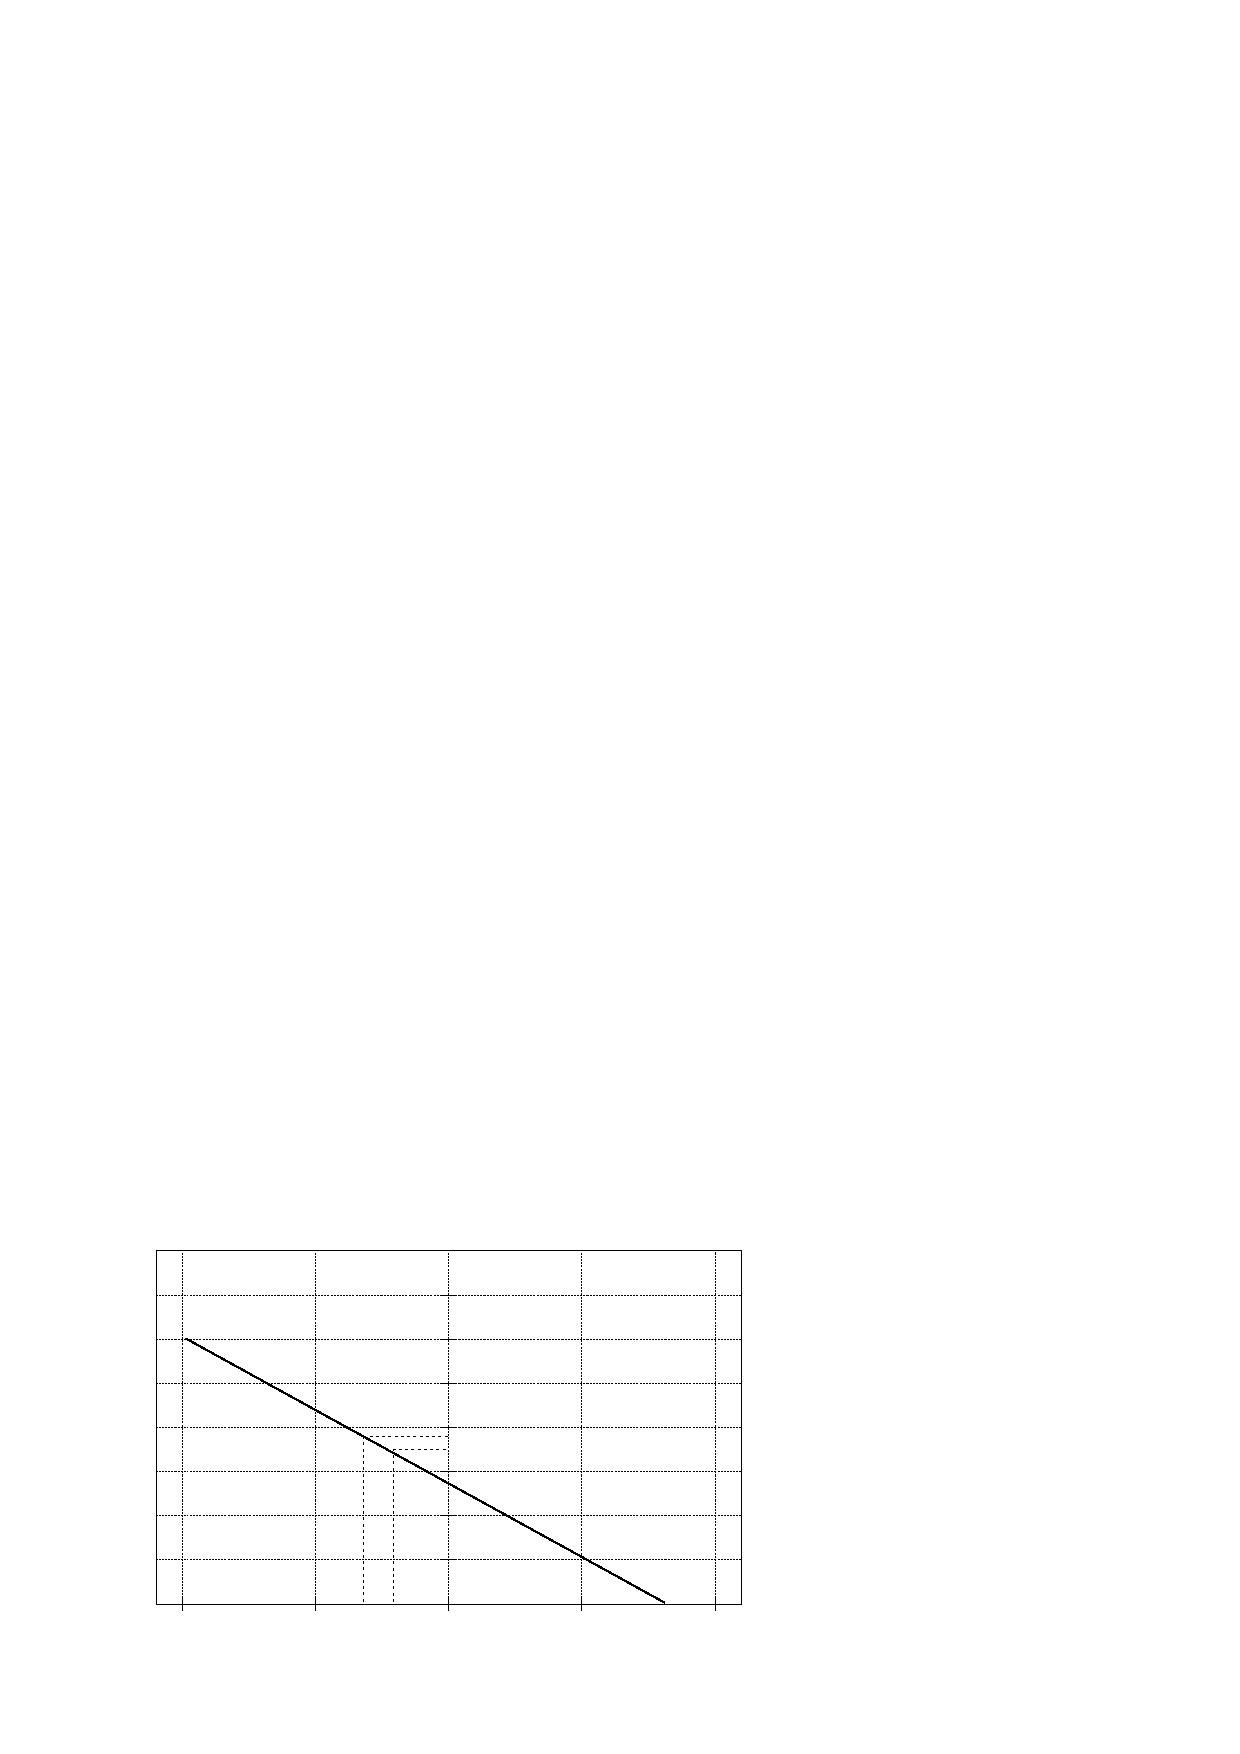
\includegraphics[width={324.00bp},height={201.50bp}]{curva3}}%
    \gplfronttext
  \end{picture}%
\endgroup

    \caption{Punto $Q$ hallado.}
    \label{curva03}
\end{figure}

Según las pruebas realizadas los valores obtenidos son:
\begin{equation*}
    \begin{split}
        R_{\text{1}} &= 1[k\Omega]\\
        R_{\text{2}} &= 100[\Omega]\\
        R_{\text{D}} &= 470[\Omega]\\
        R_{\text{S}} &= 150[\Omega]\\
\end{split}
\end{equation*}

Punto $Q$:
\begin{equation*}
    \begin{split}
        V_{\text{GS}} = -0.209\,[\text{V}]\\
        I_{\text{D}} = 7.0\,[\text{mA}]\\
    \end{split}
\end{equation*}

Rango máximo de voltaje de compuerta: 
$-0.42[{\text{V}}] < V_{\text{GS}} < 0[{\text{V}}]$.


%\section{Analisis en CA}

\subsection{BJT}
Un amplificador en emisor común (EC), tiene al emisor como terminal común, o
tierra, ante una señal de ca. Los amplificadores en EC tiene una alta ganancia de
voltaje y una alta ganancia de corriente \cite{Floyd}.

\begin{figure}[!ht]
\centering
\includegraphics[scale=0.30]{diagramas/figura17.eps}
\caption{Amplificador en emisor común.}
\label{figura17}
\end{figure}

La \textbf{figura~\ref{figura17}} muestra un amplificador en emisor común con
polarización utilizando un divisor de voltaje y capacitores de acoplamiento
$C_1$ y $C_3$ en la entrada y salida, y un capacitor de puenteo, $C_2$, del
emisor a tierra. La señal de entrada, $V_{\text{ent}}$ está acoplada
capacitivamente a la base; la señal de salida, $V_{\text{sal}}$, está acoplada
capacitivamente del colector a la carga. La salida amplificada está desfasada
$180^{\circ}$ con respecto a la entrada. Como la señal de ca se aplica a la base
como entrada y se toma en el colector como salida, el emisor es común tanto para
las señales de entrada como de salida. No hay señal en el emisor porque el
capacitor de puenteo pone efectivamente al emisor en cortocircuito con tierra a
la frecuencia de la señal. Todos los amplificadores combinan tanto la operación
en ca como en cd.

\subsubsection{Calculo de los parámetros del amplificador}
Para hallar los valores del amplificador en emisor común con divisor de voltaje
calculados en la anterior sección se calculan los siguientes valores:

\begin{enumerate}
\item Resistencia interna del generador de funciones:
\begin{equation*}
    R_s = 350[\Omega]
\end{equation*}
\item Resistencia de ca en el emisor:
\begin{equation*}
    r_e^{'} \cong \frac{25[m{\text{V}}]}{I_E}
            = \frac{\num{25e-3}[\text{V}]}{\num{36.72e-3}[\text{A}]}
            = 0.6808[\Omega]
\end{equation*}
\item Resistencia de entrada en la base:
\begin{equation*}
    R_{\text{ent(base)}} = \beta_{\text{ca}}\,r_e^{'}
                         = (302)(0.6808[\Omega])
                         = 205.6[\Omega]
\end{equation*}
\item Resistencia de entrada total vista desde la fuente:
\begin{equation*}
    R_{\text{ent(total)}} = R_1 || R_2 || R_{\text{ent(base)}}
                          = \dfrac{1}{\frac{1}{1000}+\frac{1}{200}+\frac{1}{205.6}}
                          = 92.049[\Omega]
\end{equation*}
\item Resistencia de salida:
\begin{equation*}
    R_{\text{sal}} \cong R_C
                   = 100[\Omega]
\end{equation*}
\item Atenuación de la fuente a la base:
\begin{equation*}
    A = \frac{R_s+R_{\text{ent(total)}}}{R_{\text{ent(total)}}}
      = \frac{350+92.049}{92.049}
      = 4.8023
\end{equation*}
\item Resistencia de carga:
\begin{equation*}
    R_L = 100[\Omega]
\end{equation*}
\item Resistencia en ca del colector:
\begin{equation*}
    R_c = \frac{R_C\,R_L}{R_C+R_L}
        = \frac{(100)(100)}{100+100}
        = 50[\Omega]
\end{equation*}
\item Ganancia de voltaje de la base al colector:
\begin{equation*}
    A_v = \frac{R_c}{r_e^{'}}
        = \frac{50}{0.6808}
        = 73.442
\end{equation*}
\item Ganancia de voltaje total:
\begin{equation*}
    A_v^{'} = \frac{A_v}{A}
            = \frac{73.442}{4.8023}
            = 15.293
\end{equation*}
\item Corriente total producida por la fuente:
\begin{equation*}
    I_s = \frac{V_s}{R_s+R_{\text{ent(total)}}}
        = 0.22622[m\text{A}]
\end{equation*}
\item Ganancia de corriente total:
\begin{equation*}
    A_i = \frac{I_C}{I_s}
        = \frac{\num{36.6e-3}}{\num{0.22622e-3}}
        = 161.79
\end{equation*}
\item Ganancia de potencia:
\begin{equation*}
    A_p = A_v^{'}\,A_i
        = (15.293)(161.79)
        = 2474.3
\end{equation*}
\end{enumerate}

\subsubsection{Placa de pruebas}
El circuito armado puede verse en la \textbf{figura~\ref{figura18}}, alimentado
por una fuente estable de $9[\text{V}]$ y una señal de corriente alterna
senoidal de $0.1[\text{V}]$ pico a pico.

\begin{figure}[!h]
\centering
\includegraphics[scale=0.12]{diagramas/figura18.eps}
\caption{Amplificadores en placa de pruebas.}
\label{figura18}
\end{figure}

La señal de entrada y las salidas individuales de cada amplificador puede verse
en la \textbf{figura~\ref{figura19}}.

\begin{figure}[!h]
\centering
\includegraphics[scale=0.10]{diagramas/figura19.eps}
\caption{Señales de entrada y salidas de los amplificadores.}
\label{figura19}
\end{figure}


%\subsection{FET}
La \textbf{figura~\ref{figura20}} muestra un amplificador en fuente común basado
en JFET es aquel en el que se aplica una señal de entrada de ca a la compuerta y
la señal de salida de ca se toma del drenaje. La terminal fuente es común tanto
para la señal de entrada como para la señal de salida.

\begin{figure}[!ht]
\centering
\includegraphics[scale=0.30]{diagramas/figura20.eps}
\caption{Amplificador en fuente común.}
\label{figura20}
\end{figure}

\subsubsection{Calculo de los parámetros del amplificador}
Para hallar los valores del amplificador en fuente común con divisor de voltaje
calculados en la anterior sección se calculan los siguientes valores:

\begin{enumerate}
\item Resistencia interna del generador de funciones:
\begin{equation*}
    R_i = 350[\Omega]
\end{equation*}
\item Transconductancia en $V_{\text{GS}} = 0$:
\begin{equation*}
    g_{\text{m0}} = \frac{2\,I_{\text{DSS}}}{|V_{\text{GS(corte)}}}
                  = \frac{2(\num{15.8e-3}}{|-1.037|}
                  = 0.030473[\text{S}]
\end{equation*}
\item Transconductancia en el punto Q:
\begin{equation*}
    g_{\text{m}} = g_{\text{m0}}\,\left(1 - \frac{V_{\text{GS}}}{V_{\text{GS(corte)}}}\right)
                 = 0.030473\,\left(1 - \frac{-0.209}{-1.037}\right)
                 = 0.024331[\text{S}]
\end{equation*}
\item Resistencia de entrada:
\begin{equation*}
    R_{\text{ent}} = R_1 || R_2
                   = \frac{(1000)(100)}{1000+100}
                   = 90.909[\Omega]
\end{equation*}
\item Resistencia de salida:
\begin{equation*}
    R_{\text{sal}} \cong R_D
                   = 470[\Omega]
\end{equation*}
\item Resistencia de carga:
\begin{equation*}
    R_L = 470[\Omega]
\end{equation*}
\item Ganancia de voltaje:
\begin{equation*}
    A_v = g_m\,\left(\frac{Rd\,Rl}{Rd+Rl}\right)
        = 0.024331\,\left(\frac{(470)(470)}{470+470}\right)
        = 5.7178
\end{equation*}
\end{enumerate}

\subsubsection{Placa de pruebas}
El circuito armado puede verse en la \textbf{figura~\ref{figura21}}, alimentado
por una fuente estable de $9[\text{V}]$ y una señal de corriente alterna
senoidal de $0.1[\text{V}]$ pico a pico.

\begin{figure}[!h]
\centering
\includegraphics[scale=0.10]{diagramas/figura21.eps}
\caption{Amplificador en placa de pruebas.}
\label{figura21}
\end{figure}

La señal de entrada y la salida del amplificador puede verse en la
\textbf{figura~\ref{figura22}}.

\begin{figure}[!h]
\centering
\includegraphics[scale=0.10]{diagramas/figura22.eps}
\caption{Señal de entrada y salida del amplificador.}
\label{figura22}
\end{figure}


\section{Respuesta en frecuencia}
La ganancia de voltaje y la fase de amplificadores acoplados capacitivamente se
ven afectados cuando la frecuencia de señal se encuentra por debajo de un valor
crítico. En bajas frecuencias, la reactancia de los capacitores de acoplamiento
se vuelve significativa, lo que reduce la ganancia de voltaje e incrementa el
desfasamiento \cite{Floyd}.

\subsection{BJT}

\subsubsection{Calculo de los capacitores del amplificador}
Para hallar los valores de cada capacitor del amplificador anterior sección se
calculan los siguientes valores:

\begin{enumerate}
\item Frecuencia de corte para cada capacitor del amplificador:
\begin{equation*}
    \begin{split}
        f_{\text{c2}} &= 1[k\text{Hz}]\\
        f_{\text{c1}} &= 0.2\,f_{\text{c2}} = 200[\text{Hz}]\\
        f_{\text{c3}} &= 0.2\,f_{\text{c1}} = 40[\text{Hz}]\\
    \end{split}
\end{equation*}
\item Circuito RC de entrada:
\begin{equation*}
    C_1 = \frac{1}{2\pi\,R_{\text{ent(total)}}\,f_{\text{c1}}}
    = \frac{1}{2\pi(92.049[\Omega])(200[\text{Hz}])}
    = 1.80019[\mu\text{F}]
\end{equation*}
\item Circuito RC de salida:
\begin{equation*}
    C_3 = \frac{1}{2\pi(R_C + R_L)\,f_{\text{c3}}}
        = \frac{1}{2\pi(100[\Omega]+100[\Omega])(40[\text{Hz}])}
        = 19.8944[\mu\text{F}]
\end{equation*}
\item Circuito RC de puenteo:
\begin{equation*}
    \begin{split}
        R_{\text{umbral}} &= R_1 || R_2 || R_s\\
                          &= \dfrac{1}{\frac{1}{1000}+\frac{1}{200}+\frac{1}{350}}\\
                          &= 112.90[\Omega]\\
        R_{\text{ent(emisor)}} &= r_e^{'} + \frac{R_{\text{umbral}}}{\beta_{\text{ca}}}\\
                               &= 0.6808[\Omega]+\frac{112.90[\Omega]}{302}\\
                               &= 1.0547[\Omega]\\
        C_2 &= \frac{1}{2\pi(R_{\text{ent(emisor)}} || R_E)\,f_{\text{c2}}}\\
            &= \dfrac{1}{2\pi\left(\frac{(1.0547)(22)}{1.0547+22}\right)(1000[\text{Hz}])}\\
            &= 158.141[\mu\text{F}]\\
    \end{split}
\end{equation*}
\end{enumerate}

\subsubsection{Simulación de computadora}
Se utilizó el software \emph{Quite Universal Circuit Simulator.} versión 23.3.1
para simular el circuito amplificador, este puede verse en la
\textbf{figura~\ref{figura23}}.

\begin{figure}[!h]
\centering
\includegraphics[scale=0.72]{diagramas/figura23.eps}
\caption{Simulación del amplificador.}
\label{figura23}
\end{figure}


%\subsection{FET}



\begin{thebibliography}{99}

\bibitem{Boylestad}
Robert L. Boylestad, Louis Nashelsky (2009).\\
\textbf{Electrónica: Teoría de circuitos y dispositivos electrónicos. 10ma edición.}\\
Pearson Educación

\bibitem{Floyd}
Thomas L. Floyd (2008).\\
\textbf{Dispositivos electrónicos. 8va edición.}\\
Pearson Education\\

\bibitem{Savant}
C.J. Savant Jr, Martin S. Roden, Gordon Carpenter. (1992).\\
\textbf{Diseño electrónico. Circuitos y sistemas. 2da edición.}\\
Addison-Wesley

\bibitem{2N2222A}
\textbf{2N2222A Small Signal Switching Transistor.}\\
Extraído el 3 de Noviembre del 2024, de: \\
\url{https://web.mit.edu/6.101/www/reference/2N2222A.pdf}

\bibitem{2N3819}
\textbf{2N3819 N-Channel RF Amplifier.}\\
Extraído el 11 de Noviembre del 2024, de: \\
\url{https://www.alldatasheet.com/datasheet-pdf/view/171937/FAIRCHILD/2N3819.html}

\bibitem{measuring}
\textbf{Measuring JFET Idss and Vgs(off).}\\
Extraído el 28 de Noviembre del 2024, de: \\
\url{https://therepaircafe.wordpress.com/2020/04/10/measuring-jfet-idss-and-vgsoff/}

\end{thebibliography}

\end{document}

